	%!TEX root = ./main.tex

%\documentclass[11pt, a4paper, titlepage, slovak]{book}
\documentclass[12pt, a4paper, titlepage, slovak]{book}

%Includes all neccessary packets and contains some useful commands
%!TEX root = ./main.tex

%----------------------------------------------------------------------------------
%Packages and parameters
%----------------------------------------------------------------------------------

%inputencoding for the mac
%\documentclass[slovak]{article}
\usepackage[T1]{fontenc}
\usepackage[utf8]{inputenc}
\usepackage{babel}

% =========== OLD SETTINGS =========== %
%\usepackage[utf8]{inputenc}
%\usepackage[slovak,english]{babel}
% ================================== %

%packages for mathematical symbols
\usepackage{latexsym}
\usepackage{amsmath}
\usepackage{mathtools}
\usepackage{amssymb}

\usepackage{pdfpages}

% removes 'chapter' word from titles and apply own style
\usepackage{titlesec}
\titleformat{\chapter}{\normalfont\huge\bf}{\thechapter.}{20pt}{\huge\bf}

%table design
\usepackage{booktabs}

%grahics package
\usepackage{color,graphicx}

%path to your image folder
\graphicspath{{images/}}
\usepackage{float} % package for floating images in text

%do not indent at new paragraphs but add a vertical offset
\usepackage{noindent}

%change standard fonts to Palatino and Helvetica
\usepackage{helvet}

%bibliography settings
\usepackage{natbib}
\bibliographystyle{apalike} %harvad style
%\bibliographystyle{ieeepes}

%source code listings
\usepackage{color}
\usepackage{xcolor}
\usepackage{listings}
\usepackage{caption}
\DeclareCaptionFont{white}{\color{white}}
\DeclareCaptionFormat{listing}{\colorbox{gray}{\parbox{\textwidth}{#1#2#3}}}
\captionsetup[lstlisting]{format=listing,labelfont=white,textfont=white}
\renewcommand{\lstlistingname}{Algoritmus}

%highlits
\usepackage{framed}
\definecolor{shadecolor}{rgb}{0.75,0.75,0.75}

%citation commands
\newcommand{\fullcite}{\citep} %for "Author [1980]"
\renewcommand{\citeyear}{\citeyearpar} %for "[1980]"

\usepackage{setspace}
%\doublespacing
\onehalfspacing

\usepackage[]{algorithm2e}

% change images numbering to per subsection
%\usepackage{chngcntr}
%\counterwithin{figure}{section}
%\counterwithin{table}{section}


%package for control structures
\usepackage{ifthen}

%marginpar hack --- moves margin notes to correct position
\usepackage{mparhack}

%make readable references
\usepackage[pdftex,plainpages=false,pdfpagelabels]{hyperref}


%---------------------<Layout in the style of "A Pattern Approach to Interaction Design>---------------------------

% Change page headers and footers:
\usepackage{fancyhdr}
\pagestyle{fancy}
\fancyhf{}
\fancyhead[RE]{\slshape \nouppercase{\leftmark}}    % Even page header: "page   chapter"
\fancyhead[LO]{\slshape \nouppercase{\rightmark}}   % Odd  page header: "section   page"
\fancyhead[RO,LE]{\bfseries \thepage} 
\renewcommand{\headrulewidth}{1pt}    % Underline headers
\renewcommand{\footrulewidth}{0pt}    

\fancypagestyle{plain}{               % No chapter+section on chapter start pages
\fancyhf{}
\fancyhead[RO,LE]{\bfseries \thepage}
\renewcommand{\headrulewidth}{1pt}
\renewcommand{\footrulewidth}{0pt}
}

% Left headings: "1  INTRODUCTION"
\renewcommand{\chaptermark}[1]{%
\markboth{\thechapter\ \ \ \ #1}{}}

% Right headings: "1.1  Basics"
\renewcommand{\sectionmark}[1]{%
\markright{\thesection\ \ \ \ #1}{}}


% ZMENA TABULKA ======
\renewcommand{\tablename}{Tabuľka}

% some Fancyhdr problem...
\addtolength{\headheight}{2pt} % To avoid overfull vboxes from fancyhdr

%creating a better way to change the layout for the abstract pages
\usepackage{geometry}

\titlespacing*{\chapter}{0pt}{0pt}{25pt}

\ifthenelse{\lengthtest{\paperheight=250mm}}%
{% -----------------B5 Layout-----------------
% Page layout

%\pdfpageheight250mm
%\pdfpagewidth176mm
\geometry{	b5paper,
			top = 27mm,
			footskip = 10mm,
			inner = 19mm,
			outer = 39mm,
			textheight = 175mm,
			textwidth = 84mm,
			marginparsep = 3mm,
			marginparwidth = 32mm
}
\savegeometry{myText}
% -----------------/ B5 Layout-----------------
}%
{% -----------------A4 Layout-----------------
% Page layout
\geometry{	a4paper,
			twoside,
			includemp,
			includehead,
			top = 20mm,
			headsep = 10mm,
			bindingoffset = 0mm,
			inner = 40mm,
			outer = 30mm,
			bottom = 30mm,
			marginparsep = 0mm,
			marginparwidth = 0mm
}
\savegeometry{myText}
% -----------------/ A4 Layout-----------------
}
% Abstract layout
\geometry{	marginparsep = 0mm,
			marginparwidth = 0mm
}
\savegeometry{myAbstract}
\loadgeometry{myText}


\newlength{\fullwidth} % Width of text plus margin notes
\setlength{\fullwidth}{\textwidth}
\addtolength{\fullwidth}{\marginparsep}
\addtolength{\fullwidth}{\marginparwidth}

\setlength{\headwidth}{\fullwidth} % Header stretches over margin notes


%---------------------</Layout in the style of "A Pattern Approach to Interaction Design>---------------------------


%wird fŸr die flŠchendeckende Ausgabe der Titelseite benštigt
%needed for the full-face titlepage
\usepackage{eso-pic}

%index verwenden
%make an index
\usepackage{makeidx}
\makeindex

%Index Formatierungshilfen
%formatting helpers for the index
\newcommand{\uu}[1]{\underline{#1}}
\newcommand{\ii}[1]{\textit{#1}}

%neue Definition der Index Umgebung
%redesign of the index
\renewenvironment{theindex}{%
  \vspace*{50pt}%
  {\Huge\bfseries\indexname}\par%
  \vspace*{40pt}%
  \setlength{\parskip}{0pt}%
  \setlength{\parindent}{0pt}%
  \small%
  \renewcommand{\item}{\par{}}%
  \renewcommand{\subitem}{\par\hspace{2em}- }%
}%
{}

%Maximale Gliederungstiefe, die noch ins Inhaltsverzeichnis aufgenommen wird
%maximum depth for the table of contents
\setcounter{tocdepth}{3}

%Vorschlag fŸr ein schšnes Farbschema
%Set of colors which look nice together
\usepackage{color}
\definecolor{orange_light}{rgb}{1,0.8,0.4}
\definecolor{orange_med}{rgb}{0.753,0.62,0.373}
\definecolor{orange_dark}{rgb}{0.506,0.412,0.251}

\definecolor{green_light}{rgb}{0.8,1,0.4}
\definecolor{green_med}{rgb}{0.635,0.745,0.376}
\definecolor{green_dark}{rgb}{0.435,0.498,0.255}

\definecolor{blue_light}{rgb}{0.4,0.8,1}
\definecolor{blue_med}{rgb}{0.365,0.624,0.749}
\definecolor{blue_dark}{rgb}{0.251,0.42,0.502}

\definecolor{pink_light}{rgb}{1,0.435,0.812}
\definecolor{pink_med}{rgb}{0.745,0.38,0.62}
\definecolor{pink_dark}{rgb}{0.498,0.255,0.416}

\definecolor{yellow_light}{rgb}{1,1,0.4}
\definecolor{yellow_med}{rgb}{0.757,0.745,0.373}
\definecolor{yellow_dark}{rgb}{0.506,0.49,0.251}

%blau (fŸr URLs)
%blue (for URLs)
\definecolor{blue}{rgb}{0,0,1}

%notwendig fŸr die korrekte Erkennung, auf welcher Seite sich eine Abbildung befindet.
%we need this to determine if a figure is on an odd or even page
\usepackage{chngpage}

%Hiermit kšnnen die Abbildungslegenden frei gestaltet werden
%we need this to redesign the captions
\usepackage[font=normalsize,labelfont=bf]{caption}

%Abbildungen kommen auf eine eigene Seite, wenn sie mehr als 85% des Platzes
%auf einer Seite einnehmen
%if a figure takes more than 85% of a page it will be typeset on a separate page
\renewcommand{\floatpagefraction}{0.85}

%Benštigt um gro§e Abbildungen gedreht auf eine Seite zu setzen
%we need this to rotate big figures
\usepackage[figuresright]{rotating}

%Verschiedene LŠngenma§e fŸr Textboxen
%dimensions for textboxes
\newlength{\myDefBoxWidth}
\setlength{\myDefBoxWidth}{\textwidth}
\addtolength{\myDefBoxWidth}{-4mm}
\newlength{\myBigDefBoxWidth}
\setlength{\myBigDefBoxWidth}{\fullwidth}
\addtolength{\myBigDefBoxWidth}{-4mm}

%Formathilfen fŸr MatLab Code (wer's braucht...)
%pre-defined matlab code formats
\usepackage{alltt}
\definecolor{string}{rgb}{0.7,0.0,0.0}
\definecolor{comment}{rgb}{0.13,0.54,0.13}
\definecolor{keyword}{rgb}{0.0,0.0,1.0}



%-----------------------------------------------------------------------------------------------------------------------------------------
% neue Befehle
% new commands
%-----------------------------------------------------------------------------------------------------------------------------------------

%----------------------------------------------------------------------------------

% \myBigFigure	[ LABEL_PREFIX (optional) ]
%				{ FILENAME (without extension) }
%				{ CAPTION TEXT }
%				{ SHORT VERSION OF CAPTION TEXT }
%
%Bild wird in kompletter Breite gesetzt
%picture using full width of the page
\newcommand{\myBigFigure}[4][image]
{%
\begin{figure}[ht!bp]%
%\begin{figure}[H]%
	\renewcommand{\figurename}{Obrázok}
	\checkoddpage%
	\ifcpoddpage%
		%nothing
	\else
		\hspace{-\marginparsep}\hspace{-\marginparwidth}%
	\fi
	%use minipage to center the label beneath the figure
	\begin{minipage}{\fullwidth}%
		\includegraphics[width= \fullwidth]{#2}%
		\caption[#4]{#3}%
		\label{#1_#2}%
	\end{minipage}%
\end{figure}%
}


%----------------------------------------------------------------------------------
% \myFrameBigFigure	[ LABEL_PREFIX (optional) ]
%					{ FILENAME (without extension) }
%					{ CAPTION TEXT }
%					{ SHORT VERSION OF CAPTION TEXT }
%
%Bild wird in kompletter Breite gesetzt und eingerahmt
%picture with frame using the full width of the page
\newcommand{\myFrameBigFigure}[4][image]
{
\begin{figure}[ht!bp]
%\begin{figure}[H]
	\renewcommand{\figurename}{Obrázok}
	\checkoddpage
	\ifcpoddpage
		%nothing
	\else
		\hspace{-\marginparsep}\hspace{-\marginparwidth}
	\fi
	%use minipage to center the label beneath the figure
	\begin{minipage}{\fullwidth}
	\frame{%
		\includegraphics[width= \fullwidth]{#2}%
		}
		\caption[#4]{#3}
		\label{#1_#2}
	\end{minipage}
\end{figure}
}

%----------------------------------------------------------------------------------
% \myHUGEFigure	[ LABEL_PREFIX (optional) ]
%				{ FILENAME (without extension) }
%				{ CAPTION TEXT }
%				{ SHORT VERSION OF CAPTION TEXT }
%
%Bild wird rotiert und quer in kompletter Breite gesetzt
%landscape picture using the full width of the rotated page
\newcommand{\myHugeFigure}[4][image]
{
\begin{sidewaysfigure}[t!bp]
	\checkoddpage
	\ifcpoddpage
		%nothing
		\vspace{\marginparsep}\vspace{\marginparwidth}
	\else
		%nothing
		\vspace{-\marginparsep}\vspace{-\marginparwidth}
	\fi
		\includegraphics[width= \textheight]{#2}
		\caption[#4]{#3}
		\label{#1_#2}
	
\end{sidewaysfigure}
}

%----------------------------------------------------------------------------------
% \myFigure	[ LABEL_PREFIX (optional) ]
%			{ FILENAME (without extension) }
%			{ CAPTION TEXT }
%			{ SHORT VERSION OF CAPTION TEXT }
%
%Bild wird in der Breite der textspalte gesetzt
%picture using the width of the text column
\newcommand{\myFigure}[6][image]%
{%
%\scalebox{0.5}{
\begin{figure}[#6]%
	\renewcommand{\figurename}{Obrázok}
	\begin{center}%
		\includegraphics[scale=#5]{#2}%
		\caption[#4]{#3}
		\label{#1_#2}%
	\end{center}%
\end{figure}%
}%


%----------------------------------------------------------------------------------
% \myImgRef	[ LABEL_PREFIX (optional) ]
%			{ LABEL OF THE IMAGE }
%
%referenziert das angegebene Bild
%reference to an image
\newcommand{\myImgRef}[2][image]%
{%
	\ref{#1_#2}%
}%

%----------------------------------------------------------------------------------
% \myBigTable	{ YOUR TABULAR DEFINITION }
%			{ CAPTION TEXT }
%			{ TABLE_LABLE }
%
%Tabelle wird in kompletter Breite gesetzt
%table using the full width of the page
\newcommand{\myBigTable}[3]%
{%
\begin{table}[htdp]%
	\checkoddpage%
	\ifcpoddpage%
		%nothing
	\else%
		\hspace{-\marginparsep}\hspace{-\marginparwidth}%
	\fi%
	\begin{minipage}{\fullwidth}%
		\begin{center}%
			#1%
			\caption{#2}%
			\label{#3}%
		\end{center}%	
	\end{minipage}%
\end{table}%
}%

%----------------------------------------------------------------------------------
% \myTable	{ YOUR TABULAR DEFINITION }
%			{ CAPTION TEXT }
%			{ TABLE_LABLE }
%
%Tabelle wird in der Breite der Textspalte gesetzt
%table using the width of the text column
\newcommand{\myTable}[3]%
{%
\begin{table}[htdp]%
	\begin{center}%
		#1%
		\caption{#2}%
		\label{#3}%
	\end{center}%	
\end{table}%
}%

%----------------------------------------------------------------------------------
% \myTxtRef	{ LABLE }
%
%Referenz auf Kapitel oder Abschnitte - gibt nummer und namen aus, z.B.: 5.3---"Yaddahyaddah"
%references chapters or sections, outputs number and title, e.g., 5.3---"Yaddahyaddah"
\newcommand{\myTxtRef}[1]
{%
	\ref{#1} ``\nameref{#1}''%
}

%----------------------------------------------------------------------------------
% \myTxtRefPP	{ LABLE }
%
%Referenz auf Kapitel oder Abschnitte - gibt nummer, namen und seiten aus, z.B.: 5.3---"Yaddahyaddah" (p. 45)
%references chapters or sections, outputs number and title, e.g., 5.3---"Yaddahyaddah"
\newcommand{\myTxtRefPP}[1]
{%
	\ref{#1} ``\nameref{#1}'' (p.~\pageref{#1})%
}

%----------------------------------------------------------------------------------
% \myUnderscore
%
%Setzt einen "schšnen" Unterstrich fŸr URLs
%typesets a 'nice' underscore for URLs
\newcommand{\myUnderscore}{$\underline{\hspace{0.5em}}$}

%----------------------------------------------------------------------------------
%\myTilde
%
%Setzt eine "schšne" Tilde fŸr URLs
%typesets a 'nice' tilde for URLs
\newcommand{\myTilde}{$\sim$}

%----------------------------------------------------------------------------------
% \myURL	{ TYPESET VERSION OF ANCHOR }
%			{ PRISTINE URL }
%			{ TYPESET VERSION OF URL }
%
%Setzt eine URL
%die typographisch "schšne" version erscheint in einer Fu§note,
%im Text erscheint der Ankertext, verlinkt ist die "echte" URL
%typesets a URL
%the typographically correct version appears as a footnote,
%the anchor appears in the text, the link points to the pristine URL
\newcommand{\myURL}[3]%
{%
	\textcolor{blue}{%
		\href{#2}{#1}%
	}%
	\footnote{#3}%
}

%----------------------------------------------------------------------------------
% \mySimpleURL	{ TYPESET VERSION OF ANCHOR }
%				{ PRISTINE URL }
%
%Setzt eine URL
%die URL erscheint in einer Fu§note,
%im Text erscheint der Ankertext, die URL ist verlinkt
%typesets a URL
%the URL appears as a footnote,
%the anchor appears in the text, the link points to the URL
\newcommand{\mySimpleURL}[2]%
{%
	\textcolor{blue}{%
		\href{#2}{#1}%
	}%
	\footnote{#2}%
}

%----------------------------------------------------------------------------------
% \myProjectURL	{ TYPESET VERSION OF ANCHOR }
%				{ PRISTINE URL INSIDE PROJECT DIRECTORY }
%				{ TYPESET VERSION OF URL INSIDE PROJECT DIRECTORY }
%
%Setzt eine URL auf hci/public wo die Inhalte des WebServer Ordners auf "oliver" verfŸgbar sind
%die typographisch "schšne" version erscheint in einer Fu§note,
%im Text erscheint der Ankertext, verlinkt ist die "echte" URL
%typesets a URL to hci/public from where the contents of the WebServer folder from oliver can be accessed
%the typographically correct version appears as a footnote,
%the anchor appears in the text, the link points to the pristine URL
\newcommand{\myProjectURL}[3]%
{%
	\textcolor{blue}{%
		\href{http://hci.rwth-aachen.de/public/#2}{#1}%
	}%
	\footnote{http://hci.rwth-aachen.de/public/#3}%
}

%----------------------------------------------------------------------------------
% \mnote	{ MARGIN NOTE }
%
%Setzt eine Randnotitz
%puts a comment into the margin in small sans-serif font
\newcommand{\mnote}[1]%
{%
	\leavevmode%
	\checkoddpage%
	\ifcpoddpage%
		\marginpar{\raggedright\textsf{{\footnotesize{#1}}}}%
	\else%
		\marginpar{\raggedleft\textsf{{\footnotesize{#1}}}}%
	\fi%
}
	
% leavevmode allows mnotes to be aligned with the first line of a paragraph
% NOTE: you have to put a "%" at the end of the line with the mnote, or you will get an extra blank at the beginning of the paragraph!

%----------------------------------------------------------------------------------
% \todo	{ TODO MARGIN NOTE }
%
%Setzt eine "ToDo"-Randnotitz in rot zur Erinnerung
%puts a 'todo' comment into the margin in red
\definecolor{red}{rgb}{1,0,0}
\newcommand{\todo}[1]{\mnote{\textcolor{red}{ToDo: #1}}}

%----------------------------------------------------------------------------------
% \chapterquote	{ QUOTATION }
%				{ SOURCE }
%
%Setzt ein Zitat zum Einleiten eines Kapitels
%outputs a quote with its source, can be used as an introduction to chapters
\newcommand{\chapterquote}[2]{
\begin{quotation}
    \begin{flushright}
	\noindent\emph{``{#1}''\\[1.5ex]---{#2}}
    \end{flushright}
\end{quotation}
}

%----------------------------------------------------------------------------------
% \myDefBox	{ TERM }
%			{ DEFINITION }
%
%Setzt eine Randnotitz und eine farbige Box (Textspaltenbreite),
%welche einen Begriff und seine Definition enthŠlt
%outputs a margin note and a colored box (width of the text column) containing a term and its definition
\newcommand{\myDefBox}[2]
{%
	\setlength{\fboxrule}{1mm}%
	\fcolorbox{orange_med}{orange_light}%
	{%
		\parbox{\myDefBoxWidth}{{\bfseries\scshape#1:}\\#2}%
	}%
	\mnote{Definition:\\\emph{#1}}
}

%----------------------------------------------------------------------------------
% \myBigDefBox	{ TERM }
%				{ DEFINITION }
%
%Setzt eine farbige Box (Seitenbreite), welche einen Begriff und seine Definition enthŠlt
%outputs a colored box (width of the page) containing a term and its definition
\newcommand{\myBigDefBox}[2]
{%
	\begin{figure}[h!]
	\setlength{\fboxrule}{1mm}%
	\checkoddpage%
	\ifcpoddpage%
		%nothing
	\else%
		\hspace{-\marginparsep}\hspace{-\marginparwidth}%
	\fi%
	\fcolorbox{orange_med}{orange_light}%
	{%
		\parbox{\myBigDefBoxWidth}{{\bfseries\scshape#1:}\\#2}%
	}%
	\end{figure}
}

%----------------------------------------------------------------------------------
% \myDownloadURL	{ TYPESET DOWNLOAD NAME }
%					{ PRISTINE VERSION OF FILENAME }
%					{ TYPESET VERSION OF FILENAME }
%
%Setzt eine farbige Box, welche einen Downloadlink enthŠlt
%outputs a colored box containing a download link
\newcommand{\myDownloadURL}[3]{%
\checkoddpage%
	\ifcpoddpage%
		%nothing
	\else%
		\hspace{-\marginparsep}\hspace{-\marginparwidth}%
	\fi%
\setlength{\fboxrule}{1mm}%
\fcolorbox{green_med}{green_light}{%
\begin{minipage}{\myBigDefBoxWidth}%
\begin{center}%
\myProjectURL{#1}{folder/#2}{folder/#3}%
\end{center}%
\end{minipage}%
}%
}

%----------------------------------------------------------------------------------
% \emptydoublepage
%
% Leere Doppelseite ohne Kopf- oder Fu§zeile am Ende von Kapiteln
% Clear double page without any header or footer at end of chapters
\newcommand{\emptydoublepage}{\clearpage\thispagestyle{empty}\cleardoublepage}
\newcommand{\emptysinglepage}{\clearpage\thispagestyle{empty}\clearpage}

%----------------------------------------------------------------------------------
% \pagebreak	[ SOME STRANGE LATEX VALUE ]
%
%Eklige pagebreaks fŸr den Druck (falls es nicht mehr anders geht)
%pagebreaks for the final print version (last resort weapon against wrong pagebreaks by LaTeX)
\newcommand{\PB}[1][3]
{%
	\pagebreak[#1]%
}

%----------------------------------------------------------------------------------
% \TM
%
%Setzt ein (TM) Symbol
%Places a (TM) symbol
\newcommand{\TM}
{%
	\textsuperscript{\texttrademark}%
}


% zalamovanie slov
\hyphenation{
Twitter
Twittru
map-reduce
oblastiach
korpusov
processing
modelu
vstupno
ZeroMQ
tieto
priamo
vtedy
používateľom
udalostí
}


%--------------------------------------------------------------
\begin{document}

% allow more flexible whitespaces to avoid hyphenation and overfull hboxes
\sloppy %lepsi algoritmus na zalamovanie riadkov

% 'see'-entries for the index
%!TEX root = ./main.tex
%
% This file is part of the i10 thesis template developed and used by the
% Media Computing Group at RWTH Aachen University.
% The current version of this template can be obtained at
% <http://www.media.informatik.rwth-aachen.de/karrer.html>.

\index{abbrv|see{abbreviation}}




%--------------------------------------------------------------
% uvodne strany... obal, titulka, abstrakt, uvod, ...
%--------------------------------------------------------------
\frontmatter

%use the titlepage from the 'images' directory 
\newgeometry{rmargin=20mm}
\begin{titlepage}
% centrovanie
\begin{center}                                                                                                                                                   
{\Large Slovenská technická univerzita v Bratislave} \\
{\Large Fakulta informatiky a informačných technológií} \\
\vspace*{1\baselineskip}
% cislo prace
\large {}
\vfill % vert. plnenie prazdnymi medzerami                                                                                                                                                                    

%\newpage

{{Bc. Matúš Cimerman}} \\
\vspace*{1\baselineskip}
{\LARGE {\textbf{Analýza prúdu prichádzajúcich udalostí použitím rôznych metód pre analýzu údajov}}} % nadpis
%{\huge {Analýza prúdu údajov}} % nadpis
\\
\vspace*{1\baselineskip}
%{\Large {Bakalárska práca}}\\
\textit{Diplomová práca}\\
\vfill %vert. plnenie
\end{center}
% end centrovanie
{Vedúci práce: Ing. Jakub Ševcech, PhD.}\\
\\
%\vspace*{1\baselineskip}
{december, 2016}
\end{titlepage}
\emptydoublepage

\begin{titlepage}
% centrovanie
\begin{center}                                                                                                                                                   
{\Large Slovenská technická univerzita v Bratislave} \\
{\Large Fakulta informatiky a informačných technológií} \\
\vspace*{1\baselineskip}
% cislo prace
\large {}
\vfill % vert. plnenie prazdnymi medzerami                                                                                                                                                                    


{{Bc. Matúš Cimerman}} \\
\vspace*{1\baselineskip}
{\LARGE {\textbf{Analýza prúdu prichádzajúcich udalostí použitím rôznych metód pre analýzu údajov}}} % nadpis
%{\huge {Analýza prúdu údajov}} % nadpis
\\
\vspace*{1\baselineskip}
%{\Large {Bakalárska práca}}\\
\textit{Diplomová práca}\\
\vfill %vert. plnenie
\end{center}
% end centrovanie
{Študijný program: Informačné systémy}\\
{Študijný odbor: 9.2.6 Informačné systémy}\\
{Miesto vypracovania: Ústav informatiky, informačných systémov a softvérového inžinierstva, FIIT STU v Bratislave}\\
{Vedúci práce: Ing. Jakub Ševcech, PhD.}\\
\\
{december, 2016}

\end{titlepage}
\restoregeometry
\thispagestyle{empty}
\emptydoublepage

%% This file is part of the i10 thesis template developed and used by the
% Media Computing Group at RWTH Aachen University.
% The current version of this template can be obtained at
% <http://www.media.informatik.rwth-aachen.de/karrer.html>.

~
\vfill
I hereby declare that I have created this work completely on my own and used no other sources or tools than the ones listed, and that I have marked any citations accordingly.

\begin{flushright}
\vspace{12mm}
$\overline{Bratislava, MONTH \mathit{YEAR}}$\\
\textit{YOUR NAME}
\end{flushright}

%\emptydoublepage

%pred abstrakt treba zadanie
\includepdf[pages={1}]{navrh_1.pdf}
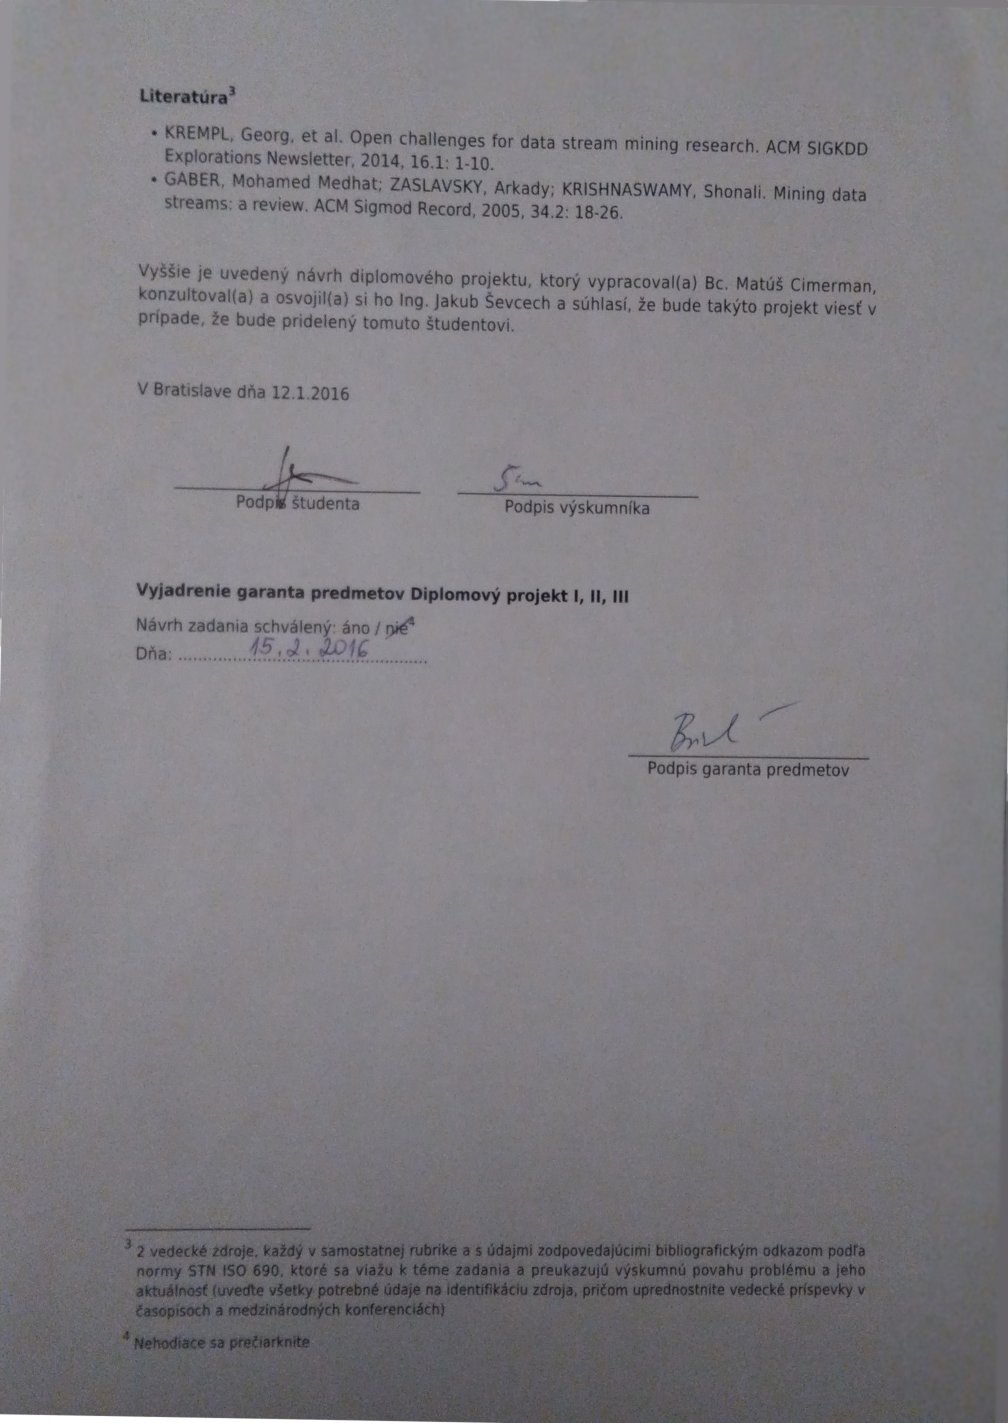
\includepdf[pages={1}]{navrh_2.pdf}

\includepdf[pages={1}]{zadanie.pdf}


%the abstract should include an english and a slovak version
\loadgeometry{myAbstract}
\chapter*{Anotácia\markboth{Abstrakt}{Abstrakt}}
%\addcontentsline{toc}{chapter}{\protect\numberline{}Abstrakt}
\label{abstrakt}
\begin{center}
\textbf{Fakulta Informatiky a Informačných Technológií}\\
\textbf{Slovenská Technická Univerzita}\\
\end{center}
\begin{tabular}{ p{15em} p{15em} }
Meno: & Bc. Matúš Cimerman\\
Vedúci diplomovej práce: & Ing. Jakub Ševcech\\
Diplomová práca: & Analýza prúdu prichádzajúcich udalostí použitím rôznych metód pre analýzu údajov\\
Študijný program: & Informačné systémy\\
Máj 2016
\end{tabular}

%here (slovak version)
Dnes môžeme pozorvať narastujúcu potrebu analyzovať dáta počas ich vzniku. Spracovanie a analýza prúdov dát predstavuje komplexnú úlohu, pričom je dôležité poskytnúť riešenie s nízkou odozvou, ktoré je odolné voči chybám.

V našej práci sa sústreďujeme na návrh súboru nástrojov, ktoré pomôžu doménovému expertovi počas analýzy dát. Doménový expert nepotrebuje mať detailné znalosti o fungovaní analytického modelu. Podobný prístup je podobný, ak chceme analyzovať statické kolekcia dát napríklad lievikovou analýzou. Študujeme možnosti použitia tradičných metód pre statické údaje v doméne analýzy prúdov dát. Našim cieľom je aplikovať metódu pre analýzu v doméne prúdu dát. Zameriavame sa pritom na jednoduchosť vybranej metódy a interpretovateľnosť výsledkov. Pre doménových expertov je nevyhnutné aby boli tieto požiadavky splnené, pretože nebudú potrebovať detailné znalosti z domén ako strojové učenie sa alebo štatistika. Naše riešenie vyhodnocujeme implementovaním softvérovej súčiastky a vybranej metódy.


%=== ENGLISH VERSION===% 
\emptydoublepage
\chapter*{Annotation\markboth{Abstract}{Abstract}}
%\addcontentsline{toc}{chapter}{\protect\numberline{}Abstract}
\label{abstract}
\begin{center}
\textbf{Faculty of Informatics and Information Technologies}\\
\textbf{Slovak University of Technology}\\
\end{center}
\begin{tabular}{ p{10em} p{15em} }
Name: & Bc. Matúš Cimerman\\
Supervisor: & Ing. Jakub Ševcech\\
Diploma thesis: & Stream analysis of incoming events using different data analysis methods\\
Course: & Information systems\\
2016, May
\end{tabular}

%here (english version)
Nowadays we can see emerging need for data analysis as data occur. Processing and analysis of data streams is a complex task, first, we particuraly need to provide low latency and fault-tolerant solution.

In our work we focus on proposal a set of tools which will help domain expert in process of data analysis. Domain expert do not need to have detailed knowledge of analytics models. Similar approach is popular when we want analyse static collections, eg. funnel analysis. We study possibilities of usage well known methods for static data analysis in domain data streams analysis. Our goal is to apply method for data analysis in domain of data streams. This approach is focused on simplicity in use of selected method and interpretability of results. It is essential for domain experts to meet these requirements because they will not need to have detailed knowledge from such a domains as machine learning or statistics. We evaluate our solution using software component implementing chosen method.

\emptydoublepage
\loadgeometry{myText}

\emptydoublepage

%acknowledgements
\loadgeometry{myAbstract}

\chapter*{Poďakovanie\markboth{Poďakovanie}{Poďakovanie}}
%\addcontentsline{toc}{chapter}{\protect\numberline{}Poďakovanie}

\vfill
Na prvom mieste vyslovujem poďakovanie vedúcemu mojej bakalárskej práce, Ing. Jakubovi Ševcechovy, za všetky jeho odborné rady, odovzdané skúsenosti a usmernenie pri tvorení práce. \\
Touto cestou taktiež vyslovujem poďakovanie všetkým výskumníkom zo skupiny PeWe, za prínosné diskusie a ich spätnú väzbu týkajúcu sa mojej práce. \\
V neposlednom rade ďakujem celej mojej rodine a priateľom.

\begin{flushright}
Matúš Cimerman
\end{flushright}


\loadgeometry{myText}


\emptydoublepage

%conventions applied in the thesis
%%!TEX root = ./main.tex
%
% This file is part of the i10 thesis template developed and used by the
% Media Computing Group at RWTH Aachen University.
% The current version of this template can be obtained at
% <http://www.media.informatik.rwth-aachen.de/karrer.html>.

\chapter*{Conventions\markboth{Conventions}{Conventions}}
\addcontentsline{toc}{chapter}{\protect\numberline{}Conventions}

Throughout this thesis we use the following conventions.



\bigskip

\emph{Text conventions}

Definitions of technical terms or short excursus are set off in coloured boxes.

\myDefBox{Excursus}
{Excursus are detailed discussions of a particular point in a book, usually in an appendix, or digressions in a written text.}

\medskip

Source code and implementation symbols are written in typewriter-style text.

\texttt{myClass}

\medskip

The whole thesis is written in Canadian English.

\medskip

Download links are set off in coloured boxes.

\myDownloadURL{File: myFile}{file_number.file}{file\myUnderscore number.file}

%\pagebreak

%\emph{Formula conventions}




%\emptydoublepage

\renewcommand{\contentsname}{Obsah}
\singlespacing
\tableofcontents

\emptydoublepage
\onehalfspacing
%\doublespacing
%
%\listoffigures
%\emptydoublepage
%
%\listoftables
%\emptydoublepage

\newtheorem{definition}{Definícia}[section]
\newtheorem{hypothesis}{Hypotéza}[section]


%--------------------------------------------------------------
% hlavny obsah
%--------------------------------------------------------------
\mainmatter

%!TEX root = ./main.tex

\chapter{Úvod}
%\label{introduction}
V súčasnosti pozorujeme zvýšený záujem o oblasť analýzy a dolovania dát. Vhodné použitie a výber metód pre spracovanie dát prináša hodnotné výstupy a náhľady pre používateľa. Výstupy môžu byť použité pre strategické rozhodnutia v podnikoch. Najčastejší postup je aplikovaním metód ako napríklad lieviková analýza alebo rozhodovacie stromy nad statickou kolekciu dát. Tento prístup má niekoľko problémov a to najmä: všetky trénovacie dáta musia byť uložené v pamäti alebo na disku, spracovanie a výpočtová náročnosť a vysporiadanie sa s trendami a zmenami v dátach. Nutnosť dáta najskôr zozbierať a uložiť, čo je dnes, kedy vznikajú milióny záznamov za deň, či hodinu, predstavuje rovnako veľký problém.\\
\\
Pod pojmom spracovanie v reálnom čase myslíme spracovanie v takmer reálnom čase, tzv. jemné (angl. soft) spracovanie v reálnom čase. Jemné spracovanie v reálnom čase znamená, že systém negarantuje spracovanie a odpoveď v stanovenom časovom limite, pričom niektoré vzorky sa môžu omeškať alebo úplne vynechať \citep{stankovic1988real}. Presné limity, do kedy sa spracovanie považuje za reálny čas závisí od problému. Niekde to môže predstavovat rádovo stotiny sekundy, v inej úlohe rádovo sekundy. V tejto práci budeme pracovať s pojmom spracovanie v reálnom čase chápajúch ako jemné spracovanie v reálnom čase.\\
\\
Pri dolovaní v prúde dát čelíme niekoľkým výzvam: objem,  rýchlosť (frekvencia) a rozmanitosť. Veľký objem dát, ktoré vznikajú veľmi rýchlo je potrebné spracovať v ohraničenom časovom intervale, často v reálnom čase. Pričom sa objem dát neustále zväčšuje, potenciálne narastá až do nekonečna. Identifikujeme niekoľko najviac zasiahnutých oblastí, ktoré sú zdrojmi týchto dát: počítačové siete, sociálne siete, Webové stránky (sledovanie správania používateľa na stránke) a Internet Vecí (angl. Internet of Things). Na informácie generované z takýchto zdrojov sa často pozeráme ako na neohraničené a potenciálne nekonečné prúdy údajov.\\
\\
Spracovanie, analýza a dolovanie v týchto prúdoch je komplexná úloha. Pre aplikácie je kritické spracovať údaje s nízkou odozvou, pričom riešenie musí byť presné, škálovateľné a odolné voči chybám. Nakoľko sú prúdy neohraničené vo veľkosti a potenciálne nekonečné, môžeme spracovať len ohraničený interval prúdu. Potom hovoríme, že dáta musia byť spracované tak ako vznikajú. Tradičné metódy a princípy pre spracovanie statickej kolekcii údajov nie sú postačujúce na takéto úlohy \citep{krempl2014open, han2011data}.
\emptydoublepage
%\chapter{Otvorené problémy pri analýze prúdu údajov}
\label{Otvorené problémy pri analýze prúdu údajov}
Dolovanie a objavovanie znalostí, alebo tiež analýza a spracovanie prúdu dát čelí trom hlavným výzvam: \textit{objem}, \textit{rýchlosť} a \textit{nestálosť} dát \citep{krempl2014open}. 

\section{Použitie tradičných metód dolovania dát a strojového učenia}

\section{Evaluácia modelov a algoritmov}

\section{Vizualizácia výsledkov používateľovi}

\section{Technické výzvy}

%\emptydoublepage
\include{methods}
\emptydoublepage
\chapter{Analytické úlohy nad prúdom dát}
\label{Analytické úlohy v prúde dát}
Spracovanie, analýza a dolovanie dát predstavuje vo všeobecnosti výzvu. Zvláštnu pozornosť si tieto úlohy vyžadujú pri spracovaní, analýze a dolovaní z prúdu prúdu udalostí. Prúd udalostí je často nazývaný \textit{prúd dát} alebo \textit{údajov}, či len skrátene \textit{prúd}. V tomto texte budeme pre jednoduchosť používať najmä termín \textit{prúd} a \textit{prúd dát} \citep{tran2014change}. Avšak môžu sa vyskytnúť aj terminý ako \textit{prúd udalostí}, \textit{sekvencia udalostí, či elementov}, pričom všetky termíny majú v tomto texte \textit{rovnaký} význam. \par
\begin{definition}{Prúd je potenciálne nekonečná sekvencia elementov \citep{tran2014change}.}
\begin{align*}
	S = \{(X_1,T_1), ..., (X_j,T_j), ...\}
\end{align*}
Kde každý element je pár $(X_j,T_j)$ kde $X_j$ je d-dimenzionálny vektor $X_j = (x_1, x_2, ..., x_d)$ prichádzajúci v čase $T_j$. $T_j$ je často nazývaný aj časová pečiatka, existujú dva typy časovej pečiatky: explicitná je generovaná keď dáta dorazia, implicitná je priradená vektoru v čase ich vzniku.
\end{definition}

% Vseobecny popis toho preco je potrebne prudove spracovanie dat
Takmer každé odvetvie dnes generuje masívne množstvo dát. Vzhľadom na ich veľký objem analytyci a doménový experti často strácajú schopnosť dolovať v celej sade dát. Stáva sa preto častým zvykom, že sa vyberie reprezentujúca vzorka, ktorej spracovanie predstavuje menšiu časovú a pamäťovú výzvu. Pri pamäťovej náročnosti hovoríme o limitoch počítača, pričom ak hovoríme o časovej náročnosti hovoríme o limitovanom čase doménového experta (čakanie na výsledok analýzy) \citep{hulten2001mining}. Predpokladajme, že bude pre doménoveho experta vysokým prínosom možnosť vykonávať analýzy nad prúdom v reálnom čase. Výstupy z takejto analýzy sú na rôznej granularite a úrovni, pričom môžu byť neskôr použité na ďalšie spracovanie alebo na priame prezentovanie výsledkov. \par

% Vyskumne vyzvy v prudoch dat vseobecne
Analýza a spracovanie prúdov dát pridáva viaceré otvorené výzvy a možnosti pre výskum \citep{krempl2014open}:
\begin{itemize}
	\item \textit{Ochrana súkromia a dôvernosti} pri analýze a dolovaní v prúde dát. Hlavným cieľom je vyvinúť metódy a techniky, ktoré neodhalia informácie a vzory, ktoré by kompromitovali potreby dôvernosti a ochrany súkromia. Dve hlavné výzvy pri analýze a dolovaní v prúdoch dát sú: \textit{vysporiadanie sa s neúplnými dátami} a \textit{uchovanie zmien (angl. concept drift) v prúde dát}.
	\item \textit{Predspracovanie} dát je dôležitou súčasťou každej reálnej aplikácie, najmä tých pre analýzu dát. Zatiaľ čo pri tradičnej analýze dát je predspracovanie vykonané jednorázovo, zvyčajne doménovým expertom. ktorý rozumie dátam. Pri prúde dát toto nieje prijateľné, pretože dáta nepretržite prichádzajú. Okrem niekoľkých štúdií \citep{zliobaite2014adaptive, anagnostopoulos2008deciding} tejto problematike nebola venovaná dostatočná pozornosť ako pri tradičnom spracovaní dát. Hlavné výzvy, ktorým treba čeliť pri predspracovaní prúdu dát sú: \textit{hluk v dátach}, \textit{outliers} a \textit{adaptívny výber vzorky}.
	\item \textit{Načasovanie a dostupnosť informácie}, väčšina algoritmov robí jednoduchý predpoklad, že prijatá informácia je kompletná, ihneď dostupná, prijatá pasívne a zadarmo. Viaceré výzvy spojené s načasovaním a dostupnosťou informácie sú formulované a nepreskúmané: \textit{spracovanie nekompletných dát}, \textit{vysporiadanie sa so skreslenou (angl. skewed) distribúciou dát} a \textit{spracovanie oneskorených dát}.
	\item \textit{Dolovanie entít a udalostí} kde entity predstavujúce prúd sú spojené do viacerých inštancií resp. štruktúrovaných informácií (napr. agregácie). Tieto entity môžu byť niekedy spojené s výskytom udalostí resp. v prúde dát. 
	\item \textit{Evaluácia algoritmov pre prúdy dát} predstavuje úplne novú výzvu v porovnaní s tradičnými metódami. Pri evaluácií v prúde dát sa musíme vysporiadať s problémami ako: \textit{zmeny (angl. concept drift}, \textit{limitovaný čas pre spracovanie vzorky}, \textit{vyvíjajúce sa skreslenie tried dát}, či \textit{oneskorenie overenia}. Tejto problematike sa v poslednej dobe venuje vyššia pozornosť, ako napríklad pre evaluáciu klasifikátorov nad prúdmi dát \citep{bifet2015efficient}.
	\item \textit{Špecializované, reaktívne a jednoduché modely} na pochopenie pre doménového experta. Tieto tri výzvy v sebe ukrývajú potrebu pre minimalizáciu závislosti na nastavení parametrov metódy, kombinácia online a offline modelov a riešenie správného problému (zmeny v prúdoch).
\end{itemize}

% Model prudu dat
\paragraph{Model prúdu dát} môže byť jeden z nasledujúcich: model časových radov, pokladničný model a model turniketu. Podľa modelu prúdu dáť existujú príslušné algoritmy, ktoré boli vytvorené pre daný model \citep{tran2014change}. Majme prúd dát $a_1, a_2, ...$, ktorý prichádza sekvenčne za sebou a popisuje podstaný signál $A$. 
V modeli časových radov každá vzorka $a_i$ sa rovná $A[i]$ pričom vzorky prichádzajú v vzostupnom poradí. Tento model je vhodný pre prúdy dát, ktoré nesú v sebe časovú postupnosť alebo je ich poradie určované časovou pečiatkou \citep{muthukrishnan2005data}.
Pri pokladničnom modeli môžme považovať množinu $U = {1, 2, ..., n}$ za element z prúdu dát. Ak uvažujeme sekvenciu $2, 1, 2, 5$ ako príklad, potom hovoríme o pokladničnom modeli. Tento model je často používaný v praxi, napríklad v prípadoch kde sled IP adries pristupuje na Web server \citep{ikonomovska2013algorithmic, muthukrishnan2005data}.
Model turniketu je veľmi podobný pokladničnému modelu. Rozdiel je v tom, že vzorka môže predstavovať aj zápornú hodnotu - analógia z reálneho sveta kedy niektorí ľudia prichádzajú a vychádzajú turniketom, počet ľudi sa mení (napr. na zjazdovke) \citep{ikonomovska2013algorithmic, muthukrishnan2005data}.

% Predspracovanie prudu dat
\paragraph{Predspracovanie prúdu}
Predspracovanie je azda najdôležitejším krokom v aplikáciach reálneho sveta a časovo najnáročnejšou úlohou pre každého analytika. Nakoľko dáta prichádzajú z nehomogénneho sveta, môžu byť zašumené, nekompletné, duplicitné alebo často obsahovať hodnoty, ktoré sa značne líšia od ostatných. Predspracovanie prúdiach údajov je potrebné čo najviac automatizovať. Existuje niekoľko známych metód a techník, ktoré sú používané pri predspracovaní prúdov dát \citep{krempl2014open, nguyen2015survey}:
\begin{itemize}
	\item \textit{Vzorkovanie}, napríklad podľa pravdepodobnostného modelu.
	\item \textit{Zahadzovania potenciálne nepotrebných vzoriek}, ak je spracujúci proces príliš zaťažený. Tu môže nastať problém, že práve zahodená vzorka bola dôležitá (zmena v dátach).
	\item \textit{Agregácia} údajov môže značne znížiť objem dát, ale môže spôsobiť problém pri potrebe pohľadu do minulosti.
	\item \textit{Aproximačné algoritmy} a ich použitie má za následok podstatné zrýchlenie spracovania a analýzy prúdov za predpokladu istej chybovosti. Chybovosť je zvačsa ohraničená.
	\item \textit{Posuvné okno}, tento prístup vznikol s potrebou analýzy definovaného časového okna z prúdiacih údajov. Výstup je teda závislí na zvolenej veľkosti okna. Problém pri tomto prístupe je práve správne nastavenie veľkosti okna tak aby sme vedeli zohladniť zmeny v prúde dát.
\end{itemize}

\par
Pri dolovaní z prúdov dát (angl. data stream mining) je potrebné aby algoritmy splňovali nasledujúce obmedzenia \citep{nguyen2015survey, wadewale2015survey}:
\begin{itemize}
	\item Jeden priechod cez dáta (angl. single-pass). Narozdiel od tradičných metód kde je možné dáta prečítať viac krát, pretože sú dáta dostupné na disku. Pri dolovaní v prúde dát nové vzorky prichádzajú kontinálne a musíme preto každú vzorku spracovať práve raz v momente keď príde.
	\item Odpoveď v reálnom čase v zmysle, že vytvorený model je pripravený kedykoľvek (angl. anytime real-time resposne) napríklad predikovať triedy nových vzoriek.
	\item K dispozícii máme len ohraničenú pamäť. Toto obmedzenie súvisí s povahou prúdou dát a to, že prúdy predstavujú potenciálne nekonečné zdroje dát.
	\item Detekcia zmien (angl. concept-drift detection) je nevyhnutná v situácii keď sa v dátach objavia nové vzory, ktoré sa menia v čase.
\end{itemize}

% Dolovanie a extrakcia informacii
\paragraph{Spracovanie, dolovanie a analýza informácií} 
Problematika spracovania, dolovania a analýzy v statickej kolekcii dát bola študovaná niekoľko dekád. Zvýšenú pozornosť začala odborná verejnosť venovať pri aplikovaní týchto úloh na prúdy dát. Niektorým z týchto úloh sa venujeme podrobne v nasledujúcich podkapitolách:
\begin{itemize}
	\item \textit{Klastrovanie}, existuje niekoľko výskumov, ktoré sa venovali špeciálne klastrovaniu implementovaním napríklad k-mediánu a inkrementálnych algoritmov.
	\item \textit{Klasifikácia}, táto úloha je dlho skúmaná s použitím rôznych metód rozhodovacích stromov.
	\item \textit{Počítanie frekvencie a opakovaní}, použitím posuvných okien a inkrementálnych algoritmov na detekciu vzorov v prúde.
	\item \textit{Analýza časových radov použitím symbolickej} reprezentácie časových radov v prúde dát. Takáto reprezentácia nám umožňuje redukciu veľkosti prenášaných dát. Táto technika pozostáva z dvoch hlavných krokov, aproximácia po častiach a následná transformácia výsledku do diskrétnych veličín.
\end{itemize}

%TODO: pridat CRISP


%%%%%%%%%%%%%%%%%%%%%%%%%%%%%%%%%%%%%%%%%%%%%%%%%
%         Dopytovanie sa v prúdoch dát          %
%%%%%%%%%%%%%%%%%%%%%%%%%%%%%%%%%%%%%%%%%%%%%%%%%
\section{Dopyty nad prúdom dát}
Vyhodnocovaniu dopytov nad statickou kolekciou dát bola venovaná značná pozornosť, ak však hovoríme o prúdoch dát dopyty musia byt vyhodnocované kontinuálne \citep{babu2001continuous, babcock2002models}. Vzniká teda nová paradigma pre interakciu s dynamicky sa meniacimi dátami, ktorú nazývame kontinuálne dopyty (angl. continious queries) \citep{babu2001continuous}. Výsledky kontinuálnych dopytov sú produkované dynamicky v čase vzniku nových dát. Príkladom použitia takýchto dopytov je napríklad sledovanie vývoja akcií burzy. Problém môže nastať pri jednorázových dopytoch, ktoré obsahujú agregačné funkcie. Pri tradičnom spracovaní dát kde sú všetky dáta uložené ako statická kolekcia, je dopyt vykonaný nad celou kolekciou. V prípade kontinuálneho dopytu je problém získať predchádzajúce dáta za predpokladu, že dáta niesú ukladané. Môžu potom nastať dva scenáre:
\begin{enumerate}
	\item agregačná funkcia je prepočítaná nad kolekciou dát, za predpokladu, že boli historické dáta ukladané.
	\item agregačná funkcia je počítaná od momentu zadanie dopytu.
\end{enumerate}
Kontinuálne dopytovanie do prúdu dát nesie so sebou nieľko výziev \citep{babcock2002models}:
\begin{itemize}
	\item \textit{Limitované pamäťové požiadavky} na algoritmy spracujúce dopyty, pretože prúd dát predstavuje potenciálne nekonečný prúd udalostí.
	\item \textit{Približné odpovede na dopyty} sú niekedy postačujúce za predpokladu, že odpoveď je dostatočné rýchla a používateľ rozumie v akej presnosti mu bola odpoveď poskytnutá. Techniky pre redukciu dimenzionality a objemu dát zahŕňajú napríklad: histogramy, náhodné vzorkovanie, symbolické vzorkovanie apod.
	\item \textit{Dopytovací jazyk} by mal byť podobný štandardu jazyka SQL. Jazyk SQL je známy deklaratívny jazyk, je široko používaný so zavedením štandardom, ktorý poskytuje flexibilitu a optimálnu evaluáciu dopytu a vykonanie nad prúdom, či datasetom. 
\end{itemize}
Výskumné práce sa tiež venovali adaptívnym kontinuálnym dopytom nad prúdmi dát. Bolo ukázané, že takýto prístup môže mať značný prínos v oblasti výkonnosti systému vďaka jeho schopnosti adaptácie na zmeny v prúde dát. Tieto vlastnosti sú dosiahnuté aplikovaním zoskupovania indexov filtrov na priebežný výber predikátov \citep{madden2002continuously}. \par
Ďalší priestor na zlepšenie výkonnosti kontinuálnych dopytov nad prúdmi dát predstavujú adaptívne filtre. Pri dopytovaní sa takmer vždy vykonáva filtrovanie dát v nejakej podobe. Tento krok filtrovania je obvykle implementovaný v systéme na spracovanie dopytov. Pre zvýšenie výkonnosti dopytov je preto možné tieto filtre presunúť priamo do zdrojov dát. Ukázalo sa, že takýto prístup môže mať pozitívny dopad na výkonnosť \citep{olston2003adaptive}. Tento prístup prinesie najmä redukciu prenášaných dát výmenou za ich nepresnosť. Problémom tejto techniky je, že je aplikovateľná len v prostredí, ktoré máme plne pod kontrolou a vieme zasahovať do všetkých jeho súčastí.



%%%%%%%%%%%%%%%%%%%%%%%%%%%%%%%%%%%%%%%%%%%%%%%%%
%               Detekcia zmien                  %
%%%%%%%%%%%%%%%%%%%%%%%%%%%%%%%%%%%%%%%%%%%%%%%%%
%TODO: doplnit typy driftov
\section{Detekcia zmien}
Detekcia zmien (angl. concept drift) zohráva, v dnešnom rýchlo sa meniacom svete, dôležitú úlohu. Zmeny nastávajú veľmi rýchlo a nečakane. Preto stúpa potreba detekcie zmeny a následná správna reakcia, ktorá vyplynie z detekovanej zmeny. Na to aby sme boli schopný na tieto zmeny adekvátne reagovať je potrebné dáta spracovávať tak ako vznikajú a pozerať sa na ne ako na prúd udalostí. Tradičné metódy pre paralelné spracovanie uvažujú len statickú kolekciu dát \citep{tran2014change}. \par
% TODO: pridat graf, ktory znazornuje rozne zmeny (nahla, inkrementalna, ...)
Detekcia zmeny predstavuje proces identifikácie zmeny aktuálneho stavu modelu voči predchádzajúcemu. Na tento objekt sa pozeráme v rôznom čase. Dôležitý rozdiel medzi zmenou a rozdielom je, že zmena hovorí o prechode modelu do iného stavu, zatiaľ čo rozdiel znamená nepodobnosť v atribútoch dvoch objektov. V kontexte prúdu, detekovanie zmeny je proces segmentácie prúdu udalostí do rôznych segmentov a identifikovanie miest kde sa zmení dynamika prúdu \citep{ross2009online}. Metóda pre detekciu zmien musí riešiť nasledujúce úlohy \citep{tran2014change}: \textit{detekcia zmeny} znamená správnu identifikáciu zmeny a \textit{lokalizácia zmeny} hovorí o identifikovaní momentu kedy zmena nastala. Týmto úloh je potrebné venovať dostatočnú pozornosť, pretože zmeny môžu byť falošné alebo dočasné čo so sebou prináša problém lokalizácie danej zmeny. Ďalší rozdiel, ktorý je potrebné zadefinovať, je medzi rozdiel detekovaním posunu pojmu (angl. concept drift). Pre lepšiu čitateľnosť tohto textu budeme pod pojmom detekcia zmeny, zmena rozumieť posun pojmu. Detekcia concept drift-u sa sústreďuje na označkované dáta, zatiaľ čo detekcia zmeny pracuje s označkovanými rovnako ako s neoznačkovanými dátami. Posun pojmu nazývame tiež časté zmeny v účelovej funkcii modelu, ktorý sa učí online. \par

Metódy pre detekovanie zmien môžme klasifikovať do nasledujúcich prístupov \citep{liu2010mining}: \textit{metódy založené na stave}, \textit{metódy sledujúce trend} a \textit{prahové metódy}. Algoritmus pre detekciu zmien by mal spĺňať aspoň nasledovné požiadavky: \textit{presnosť}, \textit{rýchlosť} a \textit{odpoveď v reálnom čase}. Algoritmus by tiež mal detekovať čo najmenej chybných zmien a čo najviac správnych presných miest zmeny. Algoritmy by mali byť prispôsobené reálnemu prostrediu a spracovaniu prúdov vysokých objemov a rýchlostí. Na obrázku \ref{fig:zmeny-vseobecny-dia} je zobrazený všeobecný diagram pre detekciu zmeny v prúde udalostí.

\myFigure{images/2_zmeny_vseobecny-diagram}{Všeobecný diagram zobrazujúci detekciu zmeny v prúde udalostí \citep{tran2014change}.}{test-dia}{0.5}{h!}\label{fig:zmeny-vseobecny-dia}

% Techniky a metody pre detekciu zmeny v prudoch
Pre detekciu zmeny v prúdoch dát bolo vyvinutých niekoľko techník a metód. Niektoré z nich nižšie podrobnejšie popisujeme.

% Charakteristika dat
\paragraph{Charakteristika dát} Metódy pre detekciu zmien môžu byť klasifikované na základe charakteru dát, s ktorými pracujú. Najčastejšie môžme prúdy klasifikovať do kategorických alebo numerických prúdov. Ak hovoríme o kategorických prúdoch, dáta obsiahnuté v prúde majú kategorický charakter, napríklad rôzny výrobcovia áut: $x \in \{Volvo, Toyota\}$. Pri numerických prúdoch dáta predstavujú numerické hodnoty $x \in {\rm I\!R}$. Pre každý takýto prúd boli vyvinuté príslušné algoritmy. Problém nastáva pri aplikáciach s dátami reálneho sveta kde prúdy často obsahujú numerické aj kategorické dáta. V takýchto situáciach má zmysel dáta rozdeliť rovnomenných skupín obsahujúce dáta rovnakého typu. Na tieto skupiny sú následne použté príslušné algoritmy. Prúdy dát sa ďalej môžu klasifikovať do označkovaných a neoznačkovaných prúdov. Neoznačkované prúdy obsahujú dáta, ktoré niesú zaradené do žiadnej triedy. Naopak označkované prúdy nesú v sebe informáciu o tom, do ktorej triedy patrí vybraný element. Rôzny charakter prúdu predstavuje rôzne zmeny a prístup na ich riešenie pri detekcii zmien v prúde \citep{tran2014change}.

% Kompletnost statistickej informacie
\paragraph{Metóda pre detekciu zmeny} V skratke DDM z anglického Drift Detection Method. Táto metóda sa zaoberá detekciou zmeny modelu. Majme prúd dát $(x_i,y_i)$ kde $x_i$ predstavuje atribúty a $y_i$ triedu vzorky. Model sa potom snaží predikovať skutočnú triedu $y_i+1$ novej vzorky. Gama a spol. založili DDM na fakte, že každá iterácia klasifikátora predikuje triedu vzorky. Klasifikátor je binárny, takže trieda môže byť len $pravda$ alebo $nepravda$. Potom, pre množinu vzoriek, chyba predstavuje náhodnú premennú z Bernoulliho pokusov (angl. Bernoulli trials). Vďaka tomu môžme chybu modelovať s bínomickým rozdelením. Nech $p$ je pravdepodobnosť zlej predikcie a $s_i$ je štandardná odchýlka vypočítaná nasledovne:
\begin{align*}
s_i = \sqrt{ \frac{p_i(1-p_i)} {i} }
\end{align*}
Pre každú vzorku z prúdu sú udržiavané dve premenné, $p_min$ a $s_min$. Ich hodnoty sú použité na výpočet varovnej hodnoty, ktorá slúži na definovanie optimálnej velkosti kontextového okna. Kontextové okno si udržiava staré vzorky, ktoré obsahujú nový kontext resp. zmenu, či posun pojmu, a minimálny počet elementov zo starého konextu. Ak sa následne zníži množstvo chybne predikovaných vzoriek, okno je zahodené ako zle identifikovaná zmena (false alarm). Naopak, ak je dosiahnutá dostatočná varovná úroveň, predtým naučený model je zahodený a vytvorený nový, ale iba zo vzoriek ktoré boli uložené do kontextového okna \citep{gama2004learning, brzezinski2010mining}.
\par
Existuje tiež rozšírenie EDDM, ktoré je modifikáciou DDM. Tento algoritmus používa rovnakú techniku varovných alarmov, ale namiesto klasifikácie chyby používa metriku množstva rozdielnych chýb. EDDM metóda dosahuje lepšie výsledky pri postupných zmenách, ale je citlivejšia na hluk v dátach \citep{wadewale2015survey}.

% ADWIN
\paragraph{ADWIN} je skratka pre algoritmus s názvom adaptívne posuvné okno (angl. adapting sliding window). Tento algoritmus je vhodný je prúdy s náhlymi zmenami. Algoritmus si udržiava okno $W$ s najnovšími vzorkami. Okno $W$ je automatický zväčšované, ak nieje detekovaná žiadna výrazná zmena v prúde a naopak zmenšované, ak bola zmena detekovaná. Obmedzenie nárastu okna do nekonečna (žiadna zmena v prúde) je možné parametrom algoritmu, ktorý bude limitovať dĺžku okna $W$. ADWIN taktiež poskytuje ohraničenie výkonu na základe množstva falošne pozitívne a falošne negatívnych vzoriek \citep{wadewale2015survey}. Základná verzia algoritmu ADWIN je vhodná pre 1-dimenzionálne dáta. Ak je potrebné detekovať zmeny pre viac-dimenzionálne dáta, potom sa vytvára paralelne niekoľko okien pre každú dimenziu dát \citep{brzezinski2010mining}.

\par
Existuje mnoho ďalších prístupov ako sa vysporiadať so zmenami v prúde, napríklad: exponenciálne váhovaný posuvný priemer, štatistické testovanie rovnomerného podielu, súborové (angl. ensemble) metódy. Popis všetkých metód je nad rámec tejto práce.



%%%%%%%%%%%%%%%%%%%%%%%%%%%%%%%%%%%%%%%%%%%%%%%%%
%             Detekcia anomálií                 %
%%%%%%%%%%%%%%%%%%%%%%%%%%%%%%%%%%%%%%%%%%%%%%%%%
\section{Detekcia anomálií}
Detekcia anomálií (angl. anomaly detection) predstavuje proces identifikácie dát, ktoré sa význačne odchyľujú (angl. deviate) od historických vzorov \citep{hodge2004survey}. Anomálie môžu spôsobovať chyby v meraní senzorov, nezvyčajné správanie systému alebo chyba pri prenose dát, či zámerné vytváranie anomálií v používateľmi generovanom obsahu. 
Takže detekcia anomálií má veľa praktického použitia napríklad v aplikáciach, ktoré dohliadajú na kvalitu a kontrolu dát \citep{hill2007real} alebo adaptívne monitorovanie sietí  \citep{hill2010anomaly}. Tieto aplikácie často kladú požiadavku aby boli anomálie detekované v čase ich v vzniku, teda v reálnom čase. Potom metódy pre detekciu anomálií musia byť rýchle vo vykonávaní a mať inkrementálny charakter. \par

V minulosti sa obvykle anomálie detekovali manuálne s pomocou vizualizačných nástrojov, ktoré doménovým expertom pomáhali v tejto úlohe. Manuálne metódy avšak zlyhávajú pri detekcií anomálií v reálnom čase. Výskumníci navrhli niekoľko metód, ktoré majú myšlienku v prístupoch strojového učenia sa a automatizovaného štatistického vyhodnocovania \citep{hill2010anomaly}: \textit{minimálny objem elipsoidu}, \textit{konvexný zvon}, \textit{najbližší sused}, \textit{zhlukovanie}, \textit{klasifikácia neurónovou sieťou}, \textit{klasifikácia metódou podporných vektorov} a \textit{rozhodovacie stromy}. Tieto metódy sú pochopiteľne rýchlejšie než manuálna detekcia, avšak jeden význačný nedostatok, bez úpravy niesú vhodné pre prúdové spracovanie v reálnom čase. Existujú napríklad rozhodovacie stromy, ktoré si dokážu budovať model inkrementálne, avšak sa líšia od dobre známych algoritmov. Táto metóda je podrobne popísana ďalej v texte.

\paragraph{Dátovo riadená metóda} (angl. data-driven), ktorú navrhli \citep{hill2010anomaly}, využíva dátovo riadený jednorozmerný autoregresívny model prúdu dát a predikčný interval (ďalej len PI) vypočítaný z posledných historických dát na identifikáciu anomálií v prúde. Dátovo riadený model časového radu je použitý, pretože je jednoduchší na implementáciu a použitie v porovnaní s ostatnými modelmi časových radov. Tento model tiež poskytuje rýchle a presné prognózy. Dáta sú potom klasifikované ako anomálie na základe toho, či sú spadnú do zvoleného intervalu PI. Metóda teda poskytuje principiálny rámec pre výber hraničného prahu kedy majú byť anomálie klasifikované. Výhoda metódy je, že nevyžaduje žiadne vzorky dát, ktoré sú vopred označkované alebo klasifikované. Je veľmi dobre škálovateľná na veľké objemy dát a vykonáva inkrementálne počítanie tak ako dáta vznikajú.
Metóda pozostáva z nasledujúcich krokov so začiatkom v čase \textit{t}:
\begin{enumerate}
	\item použi model na predikciu o krok vpred (angl. one-step-ahead), ktorý má ako vstup $\displaystyle D^t = \{x_{t-q+1}, ..., x_t\}$ \textit{q} je rôzne meranie \textit{x} v čase \textit{t} a $\displaystyle D^t$ je model predikcie. Tento model je použitý ne predikovanie hodnoty $\displaystyle \overline{x}_{t+1}$ ako očakávaná hodnota v čase \textit{t+1}.
	\item výpočet hornej a spodnej hranice kam by malo spadnúť pozorované meranie s pravdepodobnosťou \textit{p}.
	\item porovnaj pozorovanie v čase \textit{t+1}, či spadá do určeného intervalu. Ak spadne mimo intervalu, objekt je klasifikovaný ako anomália.
	\item 
		\begin{enumerate}
			\item pri stratégii metódy detekcie anomálií a zmiernenia (angl. anomaly detection and mitigation) ADAM, ak je pozorovaný objekt klasifikovaný ako anomália, modifikuj $\displaystyle D^t$ odstránením $\displaystyle x_{t-q+1}$ z konca pozorovaného okna a pridaním $\displaystyle \overline{x}_{t+1}$ na začiatok okna, čím vytvoríme $\displaystyle D^{t+1}$.
			\item pri jednoduchej stratégii detekcie anomálií (angl. anomaly detection) AD, modifikuj $\displaystyle D^t$  odstránením $\displaystyle x_{t-q+1}$ z konca okna a pridaj $\displaystyle x_{t+1}$ na začiatok okna čím vznikne $\displaystyle D^{t+1}$.
		\end{enumerate}
	\item opakuj kroky \textit{1-4}
\end{enumerate}
\paragraph{Metóda dynamických bayesových sietí} (angl. Dynamic Bayesian Networks) \citep{hill2007real} bola vytvorená pre detekciu anomálií v prúdoch zo senzorov, ktoré sú umiestnené v životnom prostredí. Bayesové siete predstavujú acyklický orientovaný graf, zobrazené na obrázku \ref{fig:anomalie-dbn}, v ktorom každý uzol obsahuje pravdepodobnostú informáciu v súvislosti k všetkým možným stavom, v ktorých sa môže premenná nachádzať. Táto informácia spolu s topológiou bayesovej siete, špecifikuje úplné spojenie distribúcie stavu premennej, pričom sada známych premmených môže byť použitá na odvodenie hodnoty neznámych premenných. Dynamické bayesové siete s topológiou, ktorá sa vyvýja v čase, pridáva nové stavové premenné pre lepšiu reprezentáciu stavu systému v aktuálnom čase \textit{t}. Stavové premmné môžeme kategorizovať ako \textit{neznáme}, ktoré predstavujú skutočný stav systému a \textit{merané}, ktoré sú nedokonalé merania. Tieto premenné môžu byť naviac diskrétne alebo spojité. Nakoľko sa veľkosť siete zväčšuje s časom, vytváranie záverov použitím celej siete by bolo neefektívne a časovo náročné. Preto boli vyvinuté aproximačné algoritmy ako \textit{Kalmanové filtrovanie} alebo \textit{Rao-Blackwellized časticové filtrovanie}. \par
Hill et al. navrhli v \citep{hill2007real} dve stratégie pre detekovanie anomálií v prúde dát:
\begin{itemize}
	\item \textit{Bayesov dôveryhodný interval} (angl. Bayesian credible interval - BCI), ktorý sleduje viacrozmernú gausovskú distribúciu lineárneho stavu premennej, ktorý korešponduje s neznámym stavom systému a jej meraným náprotivkom.
	\item \textit{Maximálne posteriori meraný status} (angl. Maximum a posteriori measurement status - MAP-ms) používa komplexnejšiu dynamickú bayseovú sieť. Princíp je rovnaký ako pri BCI, pričom MAP-ms metóda je naviac rozšírená o status (napr. anomália áno/nie), ktorý je reprezentovaný distribúciou diskrétnej premennej každého merania senzoru.
\end{itemize}
\myFigure{images/2_anomalie_DBN}{Štruktúra dnamickej bayseovej siete. Vektor $X$ reprezentuje spojitú zložku, neznáme alebo tiež nazývané skryté premenné systému a vektory $M$ predstavujú spojité pozorované premenné v čase $t$ \citep{hill2007real}.}{anomalie-dbn}{0.65}{h!}\label{fig:anomalie-dbn}


%%%%%%%%%%%%%%%%%%%%%%%%%%%%%%%%%%%%%%%%%%%%%%%%%
%                     FP                        %
%%%%%%%%%%%%%%%%%%%%%%%%%%%%%%%%%%%%%%%%%%%%%%%%%
%\section{FP} -- otazne


%%%%%%%%%%%%%%%%%%%%%%%%%%%%%%%%%%%%%%%%%%%%%%%%%
%                Zhlukovanie                    %
%%%%%%%%%%%%%%%%%%%%%%%%%%%%%%%%%%%%%%%%%%%%%%%%%
\section{Zhlukovanie}
Zhlukovanie (angl. clustering) je proces zoskupovania alebo segmentácie objektov z dátovej množiny do zhlukov (angl. cluster) na základe čŕt objektov. Cieľom je vytvoriť zhluky, kde vrámci zhluku budú objekty čo najviac podobné a objekty medzi zhlukmi čo najviac odlišné. Podobne ako pri tradičných metódach pre zhlukovanie, aj metódy pre prúdy dát môžu byť rozdelené do piatich kategórií \citep{nguyen2015survey, aggarwal2014survey}: rozdeľovacie (angl. partitioning) metódy, hierarchické (angl. hierarchical) metódy, metódy založené na hustote (angl. density-based), metódy založené na mriežke (angl. grid-based) a metódy založené na modely (angl. model-based). Algoritmus potrebuje naviac kvantifikovať mieru podobnosti, či vzdialenosti zhlukov. existujú štyri najpoužívanejšie miery pre meranie vzdialenosti: minimálna vzdialenosť (angl. single-linkage), maximálna vzdialenosť (angl. complete-linkage), primerná a stredná vzdialenosť. Zhlukovanie je príklad \textit{učenia bez učiteľa} (angl. unsupervised learning) narozdiel od klasifikácie. Metódy zhlukovania sú často používane počas predspracovania dát napríklad s cieľom redukcie dimenzionality.

\paragraph{Rozdeľovacie metódy} (angl. partitioning methods) rozdeľujú dátovú množinu o $n$ objektoch do $k$ partícií kde každá partícia predstavuje zhluk, pričom platí $k\leq n$. Parameter $k$ je obvykle definovaný používateľom vopred. Najznámejšie tradičné metódy sú $k-means$ a $k-medians$. Existujú implementácie, ktoré upravujú $k-means$ tak aby bola použiteľná na prúdy dát. Všetky tieto implementácie spracujú prúd v malých dávkach, takže nie celkom spôsobom ako je vhodné spracovať prúdy dát \citep{gaber2005mining}.
\par
Jeden z prvých algoritmov, ktoré boli navrhnuté pre prúdy dát je $STREAM$, algoritmus je rozšírením algoritmu $k-medians$. Algoritmus používa techniku rozdeľuj a panuj (angl. divide-and-conquer) s cieľom vytvárania zhlukov inkrementálne. Účelová funkcia algoritmu $STREAM$ je nasledovná:
\begin{align*}
SSQ(M,C) = \sum_{i=1}^{k} \sum_{x_j\Leftarrow c_i} dist(x_j, c_i)
\end{align*}
kde $x$ je dátová vzorka a $c$ reprezentuje zhluk (medián). Funkcia $dist$ je funkcia na meranie vzdialenosti medzi zhlukmi. Algoritmus avšak tiež spracováva dáta v malých dávkach. Na rozhodnutie o veľkosti dávky používa algoritmus $LOCALSEARCH$.

\paragraph{Metódy založené na hustote} vytvárajú profil hustoty dátovej množiny. Tento profil je následne použitý na zhlukovanie. Znamená to teda, že za zhluky považujeme miesta v priestore s vysokou hustotou objektov. Výhodou tejto metódy je, že dokáže objaviť v dátach aj neobvyklé tvary zhlukov. Najznámejšie implementácie sú $DBSCAN$ a $OPTICS$. Toto je všeobecná výhoda metód založených na hustote v porovnaní s rozdeľovacími metódami \citep{han2011data}.
\par
Algoritmus $DenStream$ je rozšírením algoritmu $DBSCAN$, ktorý je vhodný pre zhlukovanie prúdov dát. Tento algoritmus podobne ako $CluStream$ algoritmus navrhnutý Aggarwalom vytvára mikro zhluky na zachytenie informácie o prúde dát. Mikro zhluky sú kontinálne aktualizované a udržiavané v kolekcii mikro zhlukov. Algoritmus používa oslabujúci model na zníženie váh elementov v čase. Vytvárané sú tri typy mikro zhlukov: základný, potenciálny a vyčnievajúci (angl. outlier). Algoritmus potom aplikuje známy $DBSCAN$ algoritmus na vytvorené mikro zhluky, pričom zhluk vzniká z viacerých mikro zhlukov, ktoré su pokope \citep{nguyen2015survey}.
\par
Algoritmus $OPTICS-stream$ je opäť rozšírenie algoritmu $OPTICS$. Podobne ako $DenStream$ vytvára mikro zhluky a aplikuje oslabujúci model. Na vytvorenie finálnych zhlukov rovnako používa pôvodný algoritmus $OPTICS$ z vytvorených mikro zhlukov.

\paragraph{Metódy založené na modeloch} sa snažia optimalizovať podobnosť medzi dátami a statickými modelmi. Známe tradičné metódy sú napríklad $Expectation-Maximization (EM)$ a $Self-Organizing Map (SOM)$. EM je jemná (angl. soft) metóda pre zhlukovanie, SOM je metóda neurónových sietí.
\par
$SWEM$ je algoritmus rozšírený z EM algoritmu. Tento algoritmus používa posuvné okno. Každý mikro komponent je reprezentovaný n-ticou (váha, priemer, kovariančná matica). Najprv je aplikovaný algoritmus EM na získanie konvergujúcich parametrov, následne používa získané parametre ako inicializačné hodnoty pre vytvorenie modelu. SWEM tiež aplikuje oslabujúci model na expiráciu sumarizačných štatistík mikro komponentov \citep{nguyen2015survey}.
\par
Ďalším algoritmom, ktorý vytvára statický model je $GCPSOM$, ktorý je hybridným algoritmom vytvorený z $GSOM$ a $CPSOM$. Algoritmus GSOM je vyvíjajúci sa SOM kde nieje potrebné vopred definovať veľkosť mapy. Mapa GSOM dynamicky rastie podľa hodnoty akumulovaných chýb. CPSOM je bunkový pravdepodobnostný SOM, ktorý používa oslabujúce okno s cieľom redukcie váh neurónov. Teda, GCPSOM má schopnosť dynamického rastu mapy čŕt pre zhlukovanie prúdov dát a udržiavať zhluky tak ako sa prúd vyvíja v čase \citep{nguyen2015survey}.

% TODO: doplnit zhlukovacie metody
\paragraph{Hierarchické metódy}

\paragraph{Metódy založené na mriežke}






%%%%%%%%%%%%%%%%%%%%%%%%%%%%%%%%%%%%%%%%%%%%%%%%%
%                Klasifikácia                   %
%%%%%%%%%%%%%%%%%%%%%%%%%%%%%%%%%%%%%%%%%%%%%%%%%
\section{Klasifikácia}
\label{ulohy-klasifikacia}
Klasifikácia je proces hľadania všeobecného modelu, ktorý je vytvorený za základe predchádzajúcich pozorovaní. Model je potom použitý na klasifikovanie nových dát. Proces klasifikácie pozostáva z dvoch krokov: \textit{učenie} a \textit{trénovanie}. Počas učenia sa snažíme podľa algoritmu vytvoriť klasifikačný model z trénovacích dát (trénovacia množina). Počas testovania je vytvorený model použitý na klasifikovanie neoznačkovaných dát z testovacej množiny. Existujú rôzne dobre známe metódy pre klasifikáciu: rozhodovacie stromy, naivný Bayes, neurónové siete alebo k-najbližších susedov \citep{nguyen2015survey}. Niektoré z týchto metód sú v upravenej podobe vhodné na klasifikáciu prúdov dát, vybrané z nich sú detailnejšie popísané v tejto podkapitole. 
\par
Problém klasifikácie je zvyčajne formálne definovaný nasledovne: nech $A$ je trénovacia množina o $N$ prvkoch vo forme $(x,y)$ kde $y$ predstavuje skutočnú triedu vzorky a $x$ je vektor s $d$ atribútmi. Každý atribút môže nadobúdať numerické alebo kategorické hodnoty. Cieľom je vytvoriť na základe trénovacej množiny model resp. funkciu $y=f(x)$, ktorá bude predikovať triedu $y$ pre nové vzorky $x$ s vysokou presnosťou \citep{domingos2000mining}. 
\par
Väčšsina klasifikačných metód používa vzorkovanie s cieľom zvýšiť presnoť klasifikátora \citep{aggarwal2014survey, nguyen2015survey}. Často je použitá technika zásobníkového vzorkovania (angl. Reservoir sampling), ktorá umožňuje zvýšiť efektivitu klasifikátora. Myšlienka je v udržiavaní malej kontinuálnej trénovacej vzorke dát. Klasifikačný algoritmus je potom kedykoľvek aplikovaný na vzorku s cieľom vytvorenia modelu \citep{aggarwal2014survey}. Klasifikácia je problém \textit{učenia s učiteľom} (angl. supervised learning) čo znamená, že pri trénovaní sú známe skutočné triedy dátových vzoriek.

% Multi naive bayes
\paragraph{Multinomiálny naivný Bayes} je klasifikátor najčastejšie používaný na klasifikáciu dokumentov, ktorý obvykle poskytuje dobré výsledky aj čo sa týka presnosti výsledku aj rýchlosti. Túto metódu je jednoduché aplikovať v kontexte prúdu dát \citep{bifet2010sentiment}. Multinomiálny naivný Bayes sa pozerá na dokument ako na zhluk slov. Pre každú triedu $c$, $P(w|c)$, pravdepodobnosť, že slovo $w$ patrí do tejto triedy je odhadovaná z trénovacích dát jednoducho vypočítaním relatívnej početnosti každého slova v trénovacej sade pre danú triedu. Klasifikátor potrebuje naviac nepodmienenú pravdepodobnosť $P(c)$. Za predpokladu, že $\displaystyle n_{wd}$ je počet výskytov slova $w$ v dokumente $d$, pravdepodobnosť triedy $c$ z testovacieho dokumentu je nasledovaná: \newline
\begin{align*}
P(c|d) = \frac{P(c)\prod _{w \in d} P(w|c)^{n_{wd}}} {P(d)}
\end{align*}
Kde $P(d)$ je normalizačný faktor. Aby sme sa vyhli problému kedy sa trieda nevyskytuje v datasete ani jeden krát, je bežné použitie Laplacovej korekcie a nahradenie nulových početností jednotkou, resp. inicializovať početnosť každej triedy na 1 namiesto 0.

% SGD a SVM
\paragraph{Stochastický gradientný zostup a metóda podporných strojov} (angl. Stochastic Gradient Descent, SGD). Bifet a Frank v ich práci použili implementáciu tzv. vanilla stochastický gradientný zostup s pevnou rýchlosťou učenia, optimalizujúc stratu s $L_2$ penalizáciou. $L_2$ penalizácia je často používaná pri podporných vektorových strojoch (angl. Support Vector Machines, ďalej len SVM). Lineárny stroj, ktorý je často aplikovaný na problémy klasifikácie dokumentov, optimalizujeme funkciu straty nasledovne:
\begin{align*}
\frac{\lambda }{2}\left \| w \right \|^{2}+\sum [1-(yxw + b)]_{+}
\end{align*}
kde $w$ je váhovaný vektor, $b$ je sklon, $\lambda$ regulačný parameter a označenie triedy $y$ je z intervalu $\{+1, -1\}$.
\par
SVM ukazujú dobré výsledky v mnohých úlohách a problémoch strojového učenia, ak je táto metóda použitá na statické datasety. Avšak, ich použitie v neupravenej forme je problematické na prúdy dát kvoli ich časovej zložitosti $O(N^3)$ a pamäťovej zložitosti $O(N^2)$, kde $N$ je počet dátových vzoriek \citep{nguyen2015survey}. Tsang a spol. navrhli metódu jadrových vektorových strojov (angl. Core Vector Machine, CVM), ktorá používa uzavretie minimálnou guľou (angl. Minimum Enclosing Ball - MEB,v 2D priestore tiež známe ako problém pokrytia minimálnou kružicou) na redukciu časovej a pamäťovej zložitosti. Metóda StreamsSVM je rozšírením CVM a bola navrhnutá s ohľadom na spracovanie prúdov dát \citep{rai2009streamed}. StreamsSVM používa flexibilný rádius MEB, ktorý sa mení podľa nových vzoriek z prúdu dát. Výsledky sa blížia k výsledkom z optimálneho algoritmu, avšak problém tejto metódy je neschopnosť vysporiadať sa so zmenami (angl. concept-drift) v prúde dát.


% HFDT, VFDT, CVFDT
\paragraph{Rozhodovacie stromy} (angl. Decision trees) sú častou metódou používanou na klasikáciu. Modely rozhodovacích stromov dosahujú v praxi vysokú presnosť zatiaľ čo model je jednoduchý na vysvetlenie \citep{jin2003efficient, hulten2001mining, domingos2000mining, aggarwal2014survey}. Existuje niekoľko škálovateľných metód pre rozhodovacie stromy, napríklad SLIQ, RainForest alebo BOAT \citep{aggarwal2014survey}. Napriek tomu, že sú tieto metódy škálovateľné, nie sú navrhnuté a ani vhodné na použitie pre prúdy dát. Neskôr boli navrhnuté rodiny algoritmov ako ID3, ktoré boli síce navrhnuté aj s ohľadom na prúdy dát, ale problém je že neboli tak aby  zohľadnili zmeny v modely. Rozhodovacie stromy predikujú resp. klasifikujú novú vzorku do triedy $y$ podľa výsledkov testov v rozhodovacích uzloch a triedy v liste stromu do ktorého spadne vzorka.
\par
Jedna z prvých state-of-the-art metód, ktorá bola navrhnutá špecificky pre prúdy dát je \textit{Hoeffdingov strom} (angl. Hoeffding tree, ďalej len HT).  Je to najznámejšia implementácia rozhodovacích stromov v použití prúdového spracovania \citep{domingos2000mining, aggarwal2014survey, nguyen2015survey}. HT vyžaduje prečítanie každej novej vzorky z prúdu najviac jeden krát. Táto vlastnosť umožňuje použitie HT nad prúdmi dát s akceptovateľnou časovou a pamäťovou zložitosťou. Prečítané vzorky nieje potrebné ukladať na disk. HT využíva fakt, že malá vzorka dát je často postačujúca na výber optimálneho rozdelovacieho atribútu. Toto tvrdenie je matematicky podporené Hoeffdingovou mierou alebo súčtovou Chernoffovou mierou \citep{domingos2000mining, han2011data}. Rutkowski a spol. tvrdia, že stromy, ktoré používaju Hoeffdingovu mieru v skutočnosti používajú McDiarmidovu mieru a mali by sa tieto stromy nazývať McDiarmdove \citep{rutkowski2013decision}. HT dosahujú sa vo všeobecnosti asymptoticky približujú kvalitou k tým, ktoré sú vytvorené metódou pre dávkové spracovanie \citep{hall2009weka}.
\par
Predpokladajme $N$ nezávislých pozorovaní náhodnej premennej $r \in R$ kde $r$ je metrika výberu atribútu. V prípade HT to môže byť napríklad informačný zisk (angl. information gain). Ak vypočítame priemer vzorky $\overline{r}$ potom Hoeffdingova miera hovorí, že skutočný priemer $r$ je aspoň $\overline{r}-\epsilon$ s pravdepodobnosťou $1-\delta$. Pričom $\delta$ je parameter definovaný používateľom a 
\begin{align*}
\epsilon = \sqrt{ \frac{R^2ln(1/\delta)} {2n} }
\end{align*}
HT algoritmus používa Hoeffdingovu mieru na výber najmenšieho čísla $N$ - počet vzoriek potrebných v uzle na výber rozdeľovacieho atribútu. Presnejšie, v každom uzle stromu maximalizujeme $G(A_j)$ kde funkcia G predstavuje metriku kvality atribútu $A_j$ vzorky, napríklad informačný zisk. Cieľom je nájsť najmeší počet vzoriek $N$ tak aby bola splnená Hoeffdingova miera. Nech $G(A_a)$ predstavuje atribút s najvyššou hodnotou $G$ a nech $G(A_b)$ je druhý najlepší atribút. Potom ak $G(A_a) - G(A_b) > \epsilon$ môžme s istotou tvrdiť, že rozdiel je väčší ako nula. Následne vyberieme $A_a$ ako najlepší rozdeľovací atribút v danom uzle s istotu $1-\delta$. Jediné dáta, ktoré si potrebuje HT algoritmus ukladať sú postačujúce štatistiky potrebné pre rozhodovanie a výpočet Hoeffdingovej miery, sú to počítadlá $n_ijk$ pre hodnotu $v_j$ atribútu $A_i$ z triedy $y_k$. Slabá stránka tohto algoritmu je v tom, že očakáva na vstupe prúd, ktorý neobsahuje zmeny (angl. concept-drift \citep{domingos2000mining}.
\par %TODO: pridat HFDT pseudokod
Existuje niekoľko modifikácií HT algoritmu. Tá najzákladnejšia je jeho rýchla verzia (angl. Very Fast Decision Trees, VFDT) \citep{domingos2000mining}. Modifkácia HT algoritmu, ktorá sa vie vysporiadať so zmenami v prúde sa nazýva \textit{Rýchly algoritmus pre rozhodovacie stromy adaptujúci sa na zmeny} (angl. Concept-adapting Very Fast Decision Tree, CVFDT \citep{hulten2001mining}. CVFDT používa posuvné okno, pričom nevytvára pri detekovanej zmene nový model. Namiesto toho aktualizuje postačujúce štatistiky v uzloch inkrementovaním počítadiel nových vzoriek a dekrementovaním počítadiel vzoriek, ktoré vypadli z posuvného okna. Teda, ak je v prúde dát zmena, niektoré uzly stromu nemusia viac spĺňať Hoeffdingovu mieru. Keď nastane takáto situácia, alternujúci podstrom začne narastať v uzle, ktorý nesplnil Hoeffdingovu mieru. s novými vzorkami bude alternujúci podstrom rásť, zatiaľ bez toho aby bol použitý v modeli na klasifikáciu. V momente keď sa stane alternujúci podstrom presnejší ako aktuálny, starý podstrom je nahradený alternujúcim podstromom. V algoritme je možné nastaviť hraničnú hodnotu minimálneho počtu vzoriek, ktoré musí alternujúci podstrom spracovať predtým než sa pokusí nahradiť pôvodný \citep{hulten2001mining}.
\par
Ďalšou modifikáciou HT je \textit{Adaptívny sa Hoeffdingov strom} (angl. Hoeffding Adaptive Tree) predstavený Bifetom a Gavaladom v 2009. Princíp je veľmi podobný ako CVFDT, ale myšlienka je minimalizovať počet parametrov, ktoré musí používateľ nastaviť (napr. veľkosť okna $W$ je požadovaný parameter CVFDT). Adaptívny HT používa rôzne 	kritéria pre odhad potrebnej veľkosti okna automaticky, napríklad algoritmus \textit{ADWIN}. S použitím tohto kritéria používateľ nemusí zadať parameter veľkosti okna čo je obrovký prínos, pretože potrebná veľkosť sa môže meniť spolu so zmenami v prúde dát. Adaptívny HT s kritériom ADWIN dosahuje v niektorých prípadoch lepšie výsledky ako CVFDT \citep{bifet2009adaptive}.
\par
Existujú aj ďalšie odlišné metódy rozhodovacích stromov, ktoré aplikujú súborové (angl. ensemble) metódy, rôzne klasifikátory v listoch ako napríklad naivný Bayes, či stromy založené na fuzzy logike \citep{aggarwal2014survey}.


%%%%%%%%%%%%%%%%%%%%%%%%%%%%%%%%%%%%%%%%%%%%%%%%%
%                  Evaluacia                    %
%%%%%%%%%%%%%%%%%%%%%%%%%%%%%%%%%%%%%%%%%%%%%%%%%
\section{Evaluácia}
Evaluácia modelov vytvorených nad prúdmi dát je základná a dôležitá úloha pre idetifikáciu nekvalitných modelov. Toto so sebou prináša výzvy, pretože prúdy dát sú potenciálne nekončné, evaluáciu modelov je potrebné vykonávať online zatiaľ čo dáta často vytvárajú problémy, napríklad nerovnomerné rozdelenie tried v prúde dát.
% TODO: Dokoncit evaluaciu










%%%%%%%%%%%%%%%%%%%%%%%%%%%%%%%%%%%%%%%%%%%%%%%%%
%                Zhodnotenie                    %
%%%%%%%%%%%%%%%%%%%%%%%%%%%%%%%%%%%%%%%%%%%%%%%%%
\section{Zhodnotenie}
%TODO:
\emptydoublepage
\chapter{Existujúce nástroje pre analýzu prúdu udalostí}
\label{Existujúce nástroje pre analýzu prúdu udalostí}
% TODO: pridat uvod do nasledujucich nastrojov


\section{MOA}
Masívny online analyzátor (z angl. Massive Online Analysis - MOA, ďalej len MOA) je softvérové prostredie pre implementáciu algoritmov a vykonávanie experimentov pre online učenie sa z vyvýjajúcich sa prúdov dát \citep{DBLP:journals/jmlr/BifetHKP10}. MOA pozostáva z kolekcie offline a online metód a tiež nástrojov pre evaluáciu týchto metód. MOA implementuje metódy a algoritmy pre klasifikáciu, zhlukovanie prúdu, detekciu inštancií, ktoré sa vymykajú prahovým hodnotám a tiež odporúčacie systémy. Presnejšie MOA implementuje napríklad nasledujúce: stupňovanie (angl. boosting), vrecovanie (angl. bagging) a Hoeffdingove stromy, všetky metódy s a bez Naive Bayes klasifikátorom na listoch. MOA podporuje obojsmernú interakciu s nástrojom WEKA, ktorý je detailne opísaný v nasledujúcej kapitole. Na \ref{fig:moa} je možné vidieť grafické používateľské rozhranie nástroja (GUI) MOA. Okrem GUI je možné použiť konzolové a API rozhranie prostredníctvom, ktorého sa dá programovať nad rámcom/nástrojom MOA.
\par
MOA je implementovaná v programovacom jazyku Java. Za hlavnú výhodu implementácie v Jave považujú autori jej platformovú nezávislosť. MOA obsahuje tiež syntetický generátor prúdu dát, ktorým je možné modelovať tiež concept drift. V aplikácií je možné definovať pravdepodobnosť, že inštancia prúdu patrí do nového concept drift-u. Sú dostupné nasledovné generátory prúdu \citep{DBLP:journals/jmlr/BifetHKP10}: \textit{Random Tree Generator, SEA Concepts Generator, STAGGER Concepts Generator, Rotating Hyperplane, Random RBF Generator, LED Generator, Waveform Generator, and Function Generator}.
\myFigure{images/3_moa}{Hlavná obrazovka GUI nástroja MOA.}{moa}{0.45}{h!}\label{fig:moa}
\par
Evaluácia modelu je dôležitou súčasťou dolovania a analýzy dát. MOA implementuje niekoľko state-of-the-art metód pre evaluáciu modelov vytvorených príslušným algoritmom. Je možné argumentovať, že nasledujúce metódy nie sú najvhodnejšie pre evaluáciu. Toto tvrdenie je akceptovateľné, pretože evaluácia algoritmov pre dolovanie a analýzu prúdov dát je samostatná výskumna oblasť, ktorá sa ešte len vyvíja. Implementované metódy v MOA pre evaluáciu sú:
\begin{itemize}
	\item \textit{Holdout} je vhodné použiť, pretože krížová validácia môže byť často príliš časovo náročná kvôli objemu dát. Namiesto toho je použítá jediná holdout množina na vyhodnotenie kvality modelu.
	\item \textit{Prerušované testovanie-potom-trénovanie} (angl. Interleaved Test-Then-Train alebo tiež Prequential) funguje tak, že každá nová vzorka sa najprv použije na testovanie a následne na trénovanie. Vďaka tomu môže byť presnosť modelu inkrementálne aktualizovaná. Výhoda je, že nie je potrebné udržiavať holdout množinu v pamäti. 
\end{itemize}
\par
Pre spustenie grafického používateľského rozhrania nástroja MOA je potrebné stiahnuť nástroj\footnote{http://moa.cms.waikato.ac.nz/downloads/} a v príkazovom riadku spustiť nasledujúci príkaz:
\begin{lstlisting}
java -Xmx4G -cp moa.jar -javaagent:sizeofag.jar moa.gui.GUI
\end{lstlisting}
Používanie MOA z príkazového riadku:
\begin{lstlisting}
java -cp moa.jar -javaagent:sizeofag.jar moa.DoTask \
  "EvaluatePeriodicHeldOutTest -l \
	(OzaBag -l trees.HoeffdingTree -s 10)\
  -s generators.WaveformGenerator \
  -n 100000 -i 100000000 -f 1000000" > htresult.csv
\end{lstlisting}



\section{WEKA}
The Wakaito Enviroment for Knowledge Analysis (ďalej len Weka) vznikol s jednoduchým cieľom poskytunúť výskumníkom unifikovanú platformu pre prístup k state-of-the-art technikám strojového učenia sa \citep{hall2009weka}. Weka vznikla na University of Waikato na Novom Zélande v roku 1992, pričom je aktívne vyvýjaná posledných 16 rokov. Weka poskytuje kolekciu algoritmov strojového učenia sa pre úlohy dolovania v dátach. Algoritmy môžu byť priamo aplikované na datasety prostredníctvom aplikácie alebo použité vo vlastných aplikáciach volaním Java kódu. Weka obsahuje tiež nástroje na predspracovanie dát, klasifikáciu, regresiu, zhlukovanie, asociačné pravidlá a vizualizáciu. Nástroj je tiež vhodný pre navrhovanie a vývoj nových schém pre strojové učenia sa v kontexte dolovania dát. Zaujímavosťou je tiež, že Weka je nelietajúci vták, ktorý žije len na ostrove Nového Zélandu. \\

Cieľom nástroja je poskytnúť pracovný nástroj pre výskumníkov. Poskytuje napríklad (nástroj ich obsahuje omnoho viac, vymenované sú len vybrané) tieto algoritmy určené pre klasifikáciu dát:
\begin{itemize}
	\item \textit{Bayesová logistická regresia} (angl. Bayesian logistic regression), pre kategorizáciu textu s Gausovským a Laplacovým apriori.
	\item \textit{Najlepší prvý rozhodovací strom} (angl. Best-first decision tree), konštrukcia rozhodovacieho stromu so stratégiou najlepší prvý.
	\item \textit{Hybridná rozhodovacia tabuľka a naivný Bayes} (angl. Decision table naive Bayes hybrid) hybridný klasifikátor, ktorý kombinuje rozhodovacie tabuľky a metódu Naivný Bayes.
	\item \textit{Funkčné stromy} sú rozhodovacie stromy s lomeným rozdelením a lineárnymi funkciami v listoch.
\end{itemize}
Weka poskytuje tiež nástroje pre predspracovanie dát, zoznam niektorých filtrov (vymenované sú len vybrané základné filtre):
\begin{itemize}
	\item \textit{Pridanie klasifikátora}, pridá predikcie klasifikátora do datasetu.
	\item \textit{Pridanie ID} ako nového atribútu pre každý záznam datasetu.
	\item \textit{Pridanie hodnoty} chýbajúcim hodnotám z poskytnutého zoznamu.
	\item \textit{Preskupenie atribútov} preusporiadanie poradia atribútov.
	\item \textit{Numerické hodnoty na nominálne}, konverzia numerických hodnôt na nominálne.
\end{itemize}
\myFigure{images/3_weka}{Hlavná obrazovka GUI nástroja WEKA.}{weka}{0.5}{h!}\label{fig:weka}

\newpage
\section{RapidMiner Streams-Plugin}
Streams plugin poskytuje operátory RapidMiner-u pre základné budovanie blokov Streams API použítím obaľovača (angl. wrapper) na priame použitie implementácie, ktorú poskytuje Streams balík. Operátory Streams Plugin-u sú automaticky vytvorené pomocou procesora a použitím knižnice RapidMiner Beans \citep{bockermann2012processing}. Architektúra Streams Plugin-u je postavená na Streams API, ktoré bolo navrhnuté v práci Bockermanna a Bloma.
\myFigure{images/3_rapidminer}{Architektúra RapidMiner Stream Plugin-u a ďalších potrebných častí.}{rapidminer}{0.65}{h!}\label{fig:rapidminer}

\section{StreamBase}
StreamBase\footnote{http://www.streambase.com/} je platforma pre spracovanie udalostí, ktorá poskytuje vysoko-výkonný softvér pre budovanie a nasadanie systémov, ktoré analyzujú a reagujú (napr. akciami) na prúdiace dáta v reálnom čase. StreamBase poskytuje prostredie pre svižný vývoj, server pre spracovanie udalostí s nízkou odozvou a vysokou priepustnosťou a zároveň integráciu do podnikových nástrojov, napríklad pre spracovanie historických údajov. Server analyzuje prúdiace dáta a poskytuje výsledky a odpovede v reálnom čase s extrémne nízkou odozvou. Toto je dosiahnuté maximalizáciou využitia hlavnej pamäte a ostatných prostriedkov servera, zatiaľ čo sa eliminujú závislosti na ostatné aplikácie. Integrované vývojové prostredie - StreamBase Studio umožňuje programátorom jednoducho a rýchlo vytvoriť, testovat a debugovať StreamSQL aplikácie použitím grafického modelu toku vykonávania. StreamBase aplikácie sú potom skompilované a nasadené za behu servera. \\

StreamSQL je dopytovací jazyk, ktorý rozširuje štandard SQL. StreamSQL umožňuje spracovanie prúdov v reálnom čase a dopytovanie sa do nich. Základná myšlienka jazyka SQL je možnosť dopytovať sa do uložených statických kolekcií dát, StreamSQL umožňuje to isté, ale do prúdov dát. Teda, StreamSQL musí zvládnuť spracovať kontinuálny prúd udalostí a časovo orientované záznamy. StreamSQL zachováva schopnosti jazyka SQL zatiaľ čo pridáva nové možnosti ako napríklad: bohatý systém posuvných okien, možnosť miešania prúdiacich dát a statických dát a tiež možnosť pridať vlastnú logiku vo forme analytických funkcií. \\

StreamBase EventFlow je jazyk pre prúdove spracovanie vo forme tokov a operátorov ako grafických elementov. Používateľ má možnosť spájať tieto grafické elementy a vytvárať tak jednoducho topológiu pre prúdové spracovanie bez nutnosti programovania. EventFlow integruje všetky možnosti StreamSQL. \\

Použitie StreamBase sa výborne hodí pre štrukturované aplikácie "reálneho času", ktoré majú za cieľ rýchle spracovanie spolu s rýchlym prototypovaním a nasadením nových funkcionalít.
\myFigure{images/3_streambase}{Vývojové prostredie nástroja StreamBase.}{streambase}{0.55}{h!}\label{fig:streambase}

%\section{InforSphere Streams (IBM)}
\section{Spark}
Spark je klastrový výpočtový systém. Kombinuje spracovanie uložených dát v dávkovom móde so spracovaním prúdu údajov v reálnom čase \citep{cimerman2015prudy}. Cieľom Spark-u je poskytnúť rýchlu výpočtovú platformu pre analýzu dát. Spark poskytuje všeobecný model výkonávania ľubovolných dopytov, ktoré sú výkonávané v hlavnej pamäti (pokiaľ ide o prúdové spracovanie). Tento model je nazvaný \textit{Pružný distribuovaný dataset}, skr. RDD (angl. Resilient Distributed Dataset), čo je dátova abstrakcia distribuovanej pamäti. Keďže výpočet beží v hlavnej pamäti (pri prúdovom spracovaní), nie je potrebné vykonávať zápisy na disk, vďaka čomu môže byť dosiahnuté spracovanie v reálnom čase. Výpočet prebieha vo veľkom klastri uzlov s dosiahnutím odolnosti voči chybám za použitia RDD. RDD  sídli v hlavnej pamäti, ale môže byť periodicky ukladaný na disk. Vďaka distribuovanej povahe RDD môže byť stratená časť RDD obnovená z pamäti iného uzla. Samotné prúdové spracovanie nie je vykonávané správa po správe (angl. message by message), ale v mikro dávkach, ktoré môžu byť automaticky paralelne distrubované v strapci.\\
Spark Streaming\footnote{http://spark.apache.org/streaming/} alebo tiež, prúdové spracovanie, si v poslednej dobe vyžiadal špeciálnu pozornosť od tvorcom programovacieho rámca. Reagujú tým na vysoký dopyt odbornej verejnosti po prúdovom spracovaní dát, ktoré chýbalo v Spark-u. Spark Streaming poskytuje integrované rozhranie API pre rôzne programovacie jazyky, pričom v budúcnosti je snaha toto rozhranie úplne integrovať s dávakovým spracovaním, aby mohli vývojári používať rovnaké dátové typy pre rôzne typy úloh. Poskytuje tiež aspoň raz (angl. at least once) schému doručenia správ a zaručuje tak odolnosť voči chybám a prípadnej strate správy. Prúdové spracovanie v Spark-u je jednoduché integrovať spolu s dávkovým spracovaním, ktoré poskytuje, či použiť spolu s knižnicou pre strojové učenie sa. 

%Apache Flink
%Apache Storm




















\emptydoublepage
%\chapter{Implementation of proposed method}
\label{Implementation of proposed method} 

Lorem ipsum dolor sit amet, consectetur adipisicing elit, sed do eiusmod tempor incididunt ut labore et dolore magna aliqua. Ut enim ad minim veniam, quis nostrud exercitation ullamco laboris nisi ut aliquip ex ea commodo consequat. Duis aute irure dolor in reprehenderit in voluptate velit esse cillum dolore eu fugiat nulla pariatur. Excepteur sint occaecat cupidatat non proident, sunt in culpa qui officia deserunt mollit anim id est laborum. Lorem ipsum dolor sit amet, consectetur adipisicing elit, sed do eiusmod tempor incididunt ut labore et dolore magna aliqua. Ut enim ad minim veniam, quis nostrud exercitation ullamco laboris nisi ut aliquip ex ea commodo consequat. Duis aute irure dolor in reprehenderit in voluptate velit esse cillum dolore eu fugiat nulla pariatur. Excepteur sint occaecat cupidatat non proident, sunt in culpa qui officia deserunt mollit anim id est laborum. Lorem ipsum dolor sit amet, consectetur adipisicing elit, sed do eiusmod tempor incididunt ut labore et dolore magna aliqua. Ut enim ad minim veniam, quis nostrud exercitation ullamco laboris nisi ut aliquip ex ea commodo consequat. Duis aute irure dolor in reprehenderit in voluptate velit esse cillum dolore eu fugiat nulla pariatur. Excepteur sint occaecat cupidatat non proident, sunt in culpa qui officia deserunt mollit anim id est laborum.
\chapter{Klasifikácia prúdu dát použitím rozhodovacích stromov}
\label{Klasifikácia prúdu dát použitím rozhodovacích stromov}

%%%%%%%%
% Uvod %
%%%%%%%%

Klasifikácia dát je dobre známa úloha a problém dolovania, analýzy a spracovania dát. Tento problém bol veľmi dobre a podrobne študovaný pri spracovaní statickej kolekcie údajov. Pri tomto prístupe sú všetky dáta v pamäti počítača. Vybraný algoritmus potom môže pomerne "lacno" prečítať celú množinu niekoľko krát s cieľom zvýšenia presnosti a kvality výsledného modelu. Tento prístup nie je aplikovateľný pre klasifikáciu prúdov dát z nasledujúcich dôvodov:
\begin{itemize}
	\item \textit{Prúd dát je potenciálne nekonečná sekvencia udalostí}, ktoré môžu byť správne alebo chybne usporiadané v závislosti od spoľahlivosti zdroja dát. Hlavný problém tu predstavuje to, že prúd je nekonečná sekvencia udalostí. Závažnosť problému usporiadania daných udalostí, či vozriek závisí od konkrétnej úlohy analýzy prúdu dát.
	\item \textit{Obmedzená pamäť}, nieje možné všetky dáta zbierať a ukladať do pamäti. Toto obmedzenie vyplýva z prvej vlastnosti prúdov dát.
	\item \textit{Model pre klasifikácii prúdov musí byť ihneď pripravený k použitiu.} Znamená to, že hneď po tom ako sú spracované prvé dáta z prúdu, model je pripravený na použitie, napríklad klasifikovať iný prúd dát.
	\item \textit{Prúdy dát takmer vždy v sebe nesú zmeny} (angl. concept drift), na ktoré sa musí vedieť klasifikátor adaptovať. Vlasnosť klasifikačných modelov vysporiadať sa so zmenami považujeme za rozhodujúcu pri hodnotení ich kvality a použiteľnosti v praxi. Preto sa aj nami navrhovaná metóda sústreďuje na vytvorenie metódy, ktorá je schopná adaptácie na zmeny a ich adekvátne interpretovanie používateľovi. Zmeny v dátach môžu byť náhle, postupné ale môžu predstavovať aj očakávané sezónne vplyvy (napr. obdobie Vianoc z pohľadu počtu nákupov internetového obchodu).
\end{itemize}
Problém klasifikácie a jej definícia je podrobne opísaný v kapitole \ref{ulohy-klasifikacia}. V skratke, cieľom je nájsť funkciu $y = f(x)$, kde $y$ je skutočná trieda objektu/vzorky z prúdu dát a $x$ sú atribúty danej vzorky. Potom vieme pomocou funkcie $f(x)$ klasifikovať nové vzorky do triedy $y'$ s istou pravdepodobnosťou.

\par
Klasifikácia prúdov dát má zmysel často pre doménových expertov, ktorí potrebujú vytvárať detailné analýzy, či predikčné a klasifikačné modely. Pod pojmom doménový expert rozumieme človeka, ktorý rozumie analyzovaným dátam a pracuje s bežnými analytickými nástrojmi ako napríklad Google Analytics\footnote{https://www.google.com/analytics/
} alebo IBM SPSS\footnote{https://www-01.ibm.com/software/sk/analytics/spss/}. Použitie klasifikácie prúdov dát má zmysel v mnohých oblastiach a prípadoch použitia:
\begin{itemize}
	\item Detekcia podvodov pri finačných prevodoch. Je dôležité detekovať falošnú, či podvodnú platbu platobnou kartou takmer v reálnom čase pre minimalizáciu nákladov vzniknutých s jej neskorím riešením. Vytvorenie klasifikátora nad prúdmi dát ma zmysel práve preto, že transakcie predstavujú prúd dát, ktorý v sebe často nesie sezónne vzory a zmeny, na ktoré sa nevedia dobre adaptovať tradičné metódy.
	\item Klasifikácia zákaznika na webe. Toto má zmysel napríklad pre obchody ako Amazon.com. Pre takéto stránky je prínosné vedieť klasifikovať, či je navštevník webu potenciálny zakazník alebo má tendenciu odísť. Na základe týchto zistení môže majiteľ stránky vytvoriť ponuku pre zákazníka s cieľom udržať ho na stránke.
	\item Klasifikácia sieťovej prevádzky s cieľom klasifikovať potenciálne pokusy o útoky na sieť. Cieľom takejto úlohy je eliminácia útoku a stým spojená minimalizácia prestoja (angl. downtime) siete a nákladov spôsobených škodami z úspešného útoku.
\end{itemize}
Pre všetky vyššie opísané prípady použitia má zmysel zohľadniť zmeny v prúde dát v modeli. Pretože, ak sa napríklad mení správanie používateľa na webe v závislosti od zmien na stránke, napríklad v podobe zmeny dizajnu, chceme tieto zmeny odzrkadliť aj vo výslednom modeli. Rovnako ma zmysel tieto zmeny aj interpretovať prostredníctvom vizualizácie používateľovi.

\par
Existuje niekoľko dobre známych a používaných metód, niektoré z nich sú podrobne opísané v \ref{ulohy-klasifikacia}, pre klasifikáciu prúdov dát:
\begin{itemize}
	\item \textit{Hoeffdingove stromy} a ich rozšírenia, ktoré schopné adaptovať sa na zmeny (angl. concept drift) v dátach \citep{hulten2001mining, bifet2009adaptive}.
	\item \textit{Bayesová klasifikácia} a jej rozšírenia v podobe Bayesových stromov ukázali použitie najmä pri detekcii anomálií v dátach \citep{hill2007real}.
	\item \textit{Neurónové siete a evolučné metódy}. Evolučné programovanie našlo uplatnenie v stochastických optimalizačných problémoch, vlastnosti evolučných algoritmov môžu byť tiež aplikované na spracovanie prúdu dát s cieľom vysporiadať sa so zmenami v dátach. Experimentálne použitie neurónových sietí ukázalo porovnateľné výsledky s rozhodovacími stromami.
	\item \textit{Súborové metódy} (angl. ensemble), ktoré aplikujú vrecovanie (angl. bagging) a zvyšovanie (angl. boosting) s cieľom zvýšenia presnosti modelu pomocou nájdenia optimálneho nastavenia a kombinácie viacerých klasifikátorov. Náhodné lesy sú typickým príkladom súborových metód, dokážú sa vysporiadať so zmeny v dátach, pričom časová náročnosť spracovania vzorky je $O(1)$ \citep{abdulsalam2011classification}.
	\item Ďalšie metódy sú napríklad: \textit{k-najbližších susedov} a \textit{metóda podporných strojov}.
\end{itemize}

V tejto práci preto navrhujeme metódu pre klasifikáciu prúdu dát. Navrhnutá metóda môže byť použitá na akúkoľvek úlohu klasifikácie. Navrhovaná metóda používa techniku rozhodovacích stromov, je aplikovateľná na prúdy dát a model je takmer okamžite pripravený na použitie (záasadný rozdiel oproti tradičným metódam). Kladieme dôraz na spracovanie v reálnom čase, ktoré je najzákladnejšie pri spracovaní prúdov dát. Veľkú pozornosť pritom mierime na schopnosť adaptácie metódy na zmeny v dátach. Výsledný model aj s príslušnými zmenami, ktoré v dátach a modely nastali, prezentujeme používateľovi vo výslednej webovej aplikácii prostredníctvom vizualizácie. Okrem toho je našim cieľom navrhnúť metódu tak aby používateľ, ktorý je najčastejšie doménový expert, nemusel mať detailné znalosti o vnútornom fungovaní metódy.


%%%%%%%%%%%%%%%%%%%%%%%%%
% Spracovanie prudu dat %
%%%%%%%%%%%%%%%%%%%%%%%%%
\section{Spracovanie prúdu dát}
\label{method-spracovanie-prudu-dat}

Spracovaniu prúdu dát venujeme samostatnú kapitolu, pretože si zaslúži špeciálnu pozornosť a rozdielny prístup v porovnaní so spracovaním statickej kolekcii dát. Navrhovaná metóda je všeobecne použiteľná na problémy klasifikácie pre prúdy dát. Znamená to, že spracuje dáta v takmer reálnom čase, poskytne odpoveď a teda aj vytvorený model okamžite a je schopná adaptávacie na zmeny. Pre splnenie týchto požiadaviek je potrebné venovať samostatnú pozornosť spracovaniu prúdu dát, teda požadujeme aby navrhovaná metóda spĺňala nasledujúce kritéria \citep{cimerman2015prudy}:
\begin{itemize}
	\item \textit{Odolnosť voči chybám} z pohľadu architektúry spracujúcej dáta. Chybné alebo chýbajúce dáta môžu mať kritický dopad na správne fungovanie a kvalitu klasifikačného modelu.
	\item \textit{Spracovanie v reálnom čase} je opäť dôležité pre správne fugnovanie výsledného modelu, pretože model je aktualizovaný a prispôsobovaný zmenám v dátach kontiunálne. Oneskorenie niektorých správ, napríklad o 24 hodín čo je bežná prax pri ETL\footnote{ETL je proces, či architektonický vzor prenosu dát medzi viacerými častami databázových systémov  a aplikáciami, tento vzor je často používaný pre dátové sklady, skratka znamená Extrahuj, Transformuj a Načítaj (angl. Extract, Transform, Load)} procesoch, by mohlo mať nežiadúce následky vo forme skresleného modelu.
	\item \textit{Horizontálna škálovateľnosť} komponentu, ktorý spracuje prúd dát. Táto vlastnosť podporuje splnenie predchádzajúcich požiadaviek. Pod horizontálnou škálovateľnosťou chápeme to, že je možné zvýšiť výkonnosť celého systému pridaním fyzického uzla bez akýchkoľvek výpadkov. Táto požiadavka implikuje podmienku distribuovanej povahy riešenia.
\end{itemize}

S cieľom splniť tieto požiadavky sme sa rozhodli použiť nasledujúce programovacie rámce a systémy:
\begin{itemize}
	\item \textit{Storm}\footnote{http://storm.apache.org/} je programovací rámec vytvorený pre spracovanie dát v reálnom čase. Storm poskytuje možnosti škálovateľnej architektúry, ktorá je naviac odolná voči chybám na úrovni kvality dát. Programovanie nad týmto rámcom je možné v každom programocom jazyku, ktorý je možné skompilovať do Java bajtkódu a vykonávať v JVM\footnote{Virtuálny stroj Java (angl. Java virtual machine)}. Storm poskytuje aplikovať akýkoľvek programovací vzor, model ktorý poskytuje je vyjadrený, resp. vytvára acyklický orientovaný graf zostrojený z tzv. prameňov a skrutiek.
	\item \textit{Kafka}\footnote{https://kafka.apache.org/} je distribuovaná platforma pre spracovanie prúdov dát. Kafka je vhodná na budovanie apliikácií, ktoré potrebujú spracovať zdroje dát v reálnom čase a vymieňať tieto dáta medzi aplikáciami. Poskytuje možnosť publikovat (angl. publish) a predplatiť (angl. subscribe) prúdy dát. Kafka je postavená na modely fronty správ, pričom si tieto správy udržiava v pamäti a na disk ich replikuje pre prípad zlyhania.
\end{itemize}

Nasledujúci obrázok schematicky popisuje architektúru spracovania prúdu dát potrebnú pre správne fungovanie metódy pre klasifikáciu prúdu dát s použitím rozhodovacích stromov.
\myFigure{images/architecture}{Architektúra potrebná pre klasifikáciu prúdu dát v takmer reálnom čase. Architektúra pozostáva z troch úrovní. V časti predspracovania dát sú dáta zbierané zo zdroja prúdu dát a transformované do potrebnej podoby vhodnej pre ďalší krok. V kroku učenia modelu pre klasifikáciu prúdu dát je semi-automaticky vybraný vhodný algoritmus a atribúty a vytvorený klasifikačný model. Posledný krok obsahuje webovú službu, ktorá poskytuje Web API pre dotazovanie modelu. V tomto kroku tiež prezentujeme výsledky modelu v podobe vizualizácie používateľovi. Kafka je použitá na prenos správ medzi jednotlivými časťami aplikácie, správy sú rozdelené do rôznych tém podľa typu správy.}{architecture}{0.45}{h!}\label{fig:architecture}

\section{Metóda klasifikácie prúdu dát}
\label{method-klasifikacia-prudu-dat}
Cieľom je klasifikácia prúdu dát, pričom vytvorený model je pripravený na použitie takmer okamžite po prečítaní prvých vzoriek dát. Model sa tiež prispôsobuje zmenám a do istej miery sezónnym efektom v dátach. Základ metódy pre klasifikáciu sme zvolili state-of-the-art algoritmus rozhodovacích stromov, ktorý používa Hoeffdingovu mieru \citep{domingos2000mining, gaber2005mining, krempl2014open}. Hoeffdingova miera je použitá na rozhodnutie, či bol prečítaný dostatočný počet vzoriek na to aby sa mohol uzol v strome zmeniť na rozhodovací uzol. Táto miera zabezpečuje to, že sa výsledný model asymptoticky blíži svojou kvalitou k tomu, ktorý by vznikol podobnou metódou pre statické dáta. Zároveň má táto miera vlastnosť, že  dôvera v presnosť modelu exponenciálne rastie s lineárnym nárastom počtu prečítaných vzoriek. Hoeffdingova miera je definovaná používateľom parametrom spoľahlivosti $\delta$, kde spoľahlivosť je $(1-\delta) \in <0,1>$. Metrika kvality vzorky $G$ môže byť použitá ľubovoľná, napríklad informačný zisk (angl. information gain).
\par
Metóda potrebuje na trénovanie označkované numerické alebo kategorické dáta do viacerých tried. Dáta musia byť vo forme n-tíc $(x_1, x_2, ..., x_n | y)$ kde $x$ sú atribúty vzorky a $y$ skutočná trieda vzorky. Nami vybraný potrebuje len minimum parametrov, ktoré je potrebné nastaviť pre správne fungovanie. Jedným z nich metódy je minimálny počet spracovaných vzoriek pred vytvorením prvého modelu. Týmto je možné minimalizovať prvotnú nepresnosť počiatočného modelu. Výsledný model je jednoduchý na reprezentáciu vďaka možnosti jeho intuitívnej interpretácii rozhodovacím stromom. Rozhodovací strom pozostáva z rozdeľovacích uzlov (angl. split node), tiež niekedy nazývané testovacie uzly, a listov (angl. leaf). V rozhodovacích uzloch sa vykonáva testovanie vzorky a jej posunutie do jednej z nasledujúcich vetiev alebo listu stromu. Ak vzorka narazí na list znamená to, že bola klasifikovaná do istej triedy, ktorú opisuje daný list. Takto vytvorený model je použiteľný na klasifikáciu v rôznych aplikáciách.
\par
Problémom rozhodovacích stromov je najmä ich šírka. Klasifikátory, ktoré používajú modely a algoritmy rozhodovacích stromov môžu podľa dát byť priveľmi široké. Tento problém môže mať za následok preučenie (angl. overfitting) modelu, ktorý bude vedieť klasifikovať veľmi dobre trénovacie dáta, resp. dáta zo začiatku prúdu, ale na nových dátach bude veľmi nepresný. Tento problém nastáva najmä pri spojitých číselných atribútoch a ich nerovnomernej distribúcii. Existuje niekoľko známych spôsobov ako sa stýmto nežiadúcim javom vysporiadať, jedným z nich je pre-prerezávanie (angl. pre-pruning) stromu. Tento spôsob aplikujeme aj v našej metóde priadním nulového atribútu $X_0$ do každého uzla, ktorý spočíva v nerozdeľovaní daného uzla. Takže uzol sa stane rozhodovacím iba, ak je metrika $G$, so spoľahlivosťou $1-\delta$, lepšia ako keby sa uzol nezmenil na rozhodovací.
\par
V našich experimentoch sa, ale ukázalo, že pre-prerezávanie nieje dostatočný spôsob pre redukciu šírky stromu. Navrhujeme preto použiť metódy pre výber významných atribútov. Znamená to teda, že nebudú použité všetky atribúty pre učenie modelu a jeho následné použitie. Na takúto významovú analýzu je možné použiť napríklad náhodné lesy. Náhodné lesy vytvárajú veľa jednoduchých stromov, kde každý strom obsahuje práve jeden rozhodovací uzol. Následné sa zvolenou metrikou vyberú najvýznamnejšie atribúty a tie budú použité pre trénovanie a použitie klasifikátora. Okrem použitia náhodných lesov navrhujeme použiť histogrami pre spojité numerické atribúty s cieľom redukovať šírku stromu.
\par
Nami navrhovaná metóda sa musí vysporiadať so zmenami v dátach, pretože tie nesú v sebe takmer všetky prúdy dát. Zmeny môžu mať rôzny charakter, napríklad náhly kedy zmena nastane nečakane alebo postupný kedy sa zmena deje dlhú dobu a pomaly. Výsledný model musí pre udržanie svojej presnosti zohladniť tieto zmeny. Metóda používa algoritmus \textit{ADWIN} z anglického Adaptive Windowing \citep{Hutchison2009}. Tento algoritmus nepožaduje žiadne nastavenia parametrov používateľom ako napríklad veľkosť posuvného okna. Jediným parametrom je hodnota istoty $\delta$ s akou bude algoritmus detekovať zmeny v prúde dát. Myšlienka ADWIN spočíva v tom, že nenenastala žiadna zmena v priemernej hodnote vybranej metriky v okne. Ak je detekovaná zmena, v uzle začne narastať alternujúci podstrom. Tento podstrom musí spracovať definovaný minimálny počet vzoriek. Potom, ak je kvalita podstromu vyššia ako kvalita podstromu, z ktorého začal narastať, starý podstrom je nahradený alternujúcim podstromom. Naraz môže existovať niekoľko alternujúcich podstromov, pričom môže nastať situácia kedy ani jeden z nich nebude mať vyššiu kvalitu a nesplní Hoeffdingovu mieru preto aby nahradil starý podstrom. Výsledok tohto algoritmu chceme detailne prezentovať používateľovi vo forme vizualizácie, ktorá je detailnejšie popísaná v nasledujúcej podkapitole. 



%%%%%%%%%%%%%%%%%%%%%%%%%%%%%%%%%%%%%%%
% Prezentacia vysledkov pouzivatelovi %
%%%%%%%%%%%%%%%%%%%%%%%%%%%%%%%%%%%%%%%

\section{Prezentácia výsledkov používateľovi}
\label{my-method-prezentacia-vysledkov}
V situácii keď potrebuje doménovy expert vytvoriť klasifikačný model s použitím dát reálneho sveta, je často potrebná najprv detailná znalosť dát, ktorú doménový expert, predpokladáme má.  Následne preto, aby vedel vytvoriť správny model potrebuje mať detailné znalosti o fungovaní klasifikačných metód a algoritmov. Cieľom našej metódy je odbremeniť experta od nutnosti mať detailné znalosti o fungovaní modelu a algoritmov. Zameriavame sa teda na prezentáciu dôležitých informácií, ktoré potrebuje pre správne pochopenie modelu a následné rozhodnutia. Výber atribútov a algoritmov, ktoré budú použité na trénovanie modelu je bez nutnosti interakcie používateľa v zmysle nastavovania parametrov a výberu metódy. 
\par
Pretože používateľ nemusí mať detailné znalosti o fungovaní algoritmov a klasifikačných metód, je dôležité vysvetlenie výsledného modelu. Znamená to, že je dôležité aby pre používateľa nebol vzniknutý model len čierna skrinka (angl. black-box), ktorá s nejakou úspešnosťou dokáže klasifikovať prúdy dát. Navrhujeme preto vizualizáciu výsledného modelu. Vizualizácia je vo forme rozhodovacieho stromu, ktorý je jednoduchý na pochopenie aj bez predchádzajúcich znalostí o rozhodovacích stromov \citep{nguyen2015survey}. Sústreďujeme sa tiež na zobrazenie zmien (angl. concept drift) v dátach resp. zmenách, ktoré sa odzrkadlia aj v modely. Zmeny samotného modelu vizualizujeme ako animáciu, ktorú je možné spustiť a pozorovať vývoj stromu. Ďalej poskytujeme náhľad vo forme čiarového grafu na kvalitu alternujúcich podstromov, ktoré boli vytvorené pri detekovaní zmeny. Na nasledujúcom obrázku je zobrazený prvý prototyp vizualizácie modelu rozhodovacieho stromu, zmeny sú vizualizované pomocou animácie.
\myFigure{images/exp-vis-prototype}{Prototyp vizualizácie modelu rozhodovacieho stromu s použitím Hoeffdingovej miery. Veľkosť rozhodovacích uzlov znázorňuje počet potrebných vzoriek na výber najlepšieho atribútu, čím väčší je kruh, tým viac vzoriek bolo potrebných pre splnenie Hoeffdingovej miery. S vizualizáciou je možné interagovať myšou.}{exp-vis-prototype}{0.35}{h!}\label{fig:exp-vis-prototype}
Pomocou týchto vizualizácií chceme prezentovať výsedky našej klasifikačnej metódy používateľovi. Prezentované výsledky by mali byť jednoduché na pochopenie aj bez detailných znalostí o fungovaní metódy a algoritmov. Overenie použiteľnosti a miery pochopenia prezentovaných výsledkov overujeme detailnými používateľskými štúdiami a vyhodnotením tromi doménovými expertami (majú znalosti o fungovaní metódy a algoritmov). 


\section{Vyhodnotenie a experimenty}
Pre kvantifikovanie správneho fungovania nami navrhovanej metódy navrhujeme viaceré experimenty. Prvým z experimentov je vyhodnotenie integrácie časti spracovania prúdu dát s našou metódou. Pri tomto vyhodnocovaní sa budeme pozerať na výkonnostné metriky, ktoré hovoria o priepustnosti a výkone tejto časti aplikácie. Zaujíma nás hlavne odolnosť voči chýbam, spracovanie v reálnom čase a zaťaženie procesoru a pamäte v závislosti na objeme dát.
\par
Vyhodnotenie samotnej metódy pre klasifikáciu prúdu dát nás zaujímajú bežné metriky používané pri vyhodnocovaní modelov strojové učenie, ako napríklad presnosť (angl. precision) a pokrytie (angl. recall). Keďže ide o klasifikovanie prúdu dát, zameriavame sa tiež na nasledujúce metriky:
\begin{itemize}
	\item \textit{Kappa štatistiky}, ktoré dobre vyjadrujú presnosť klasifikátora nestabilné prúdy dát.
	\item \textit{Najprv test-potom-trénovanie} (angl. Test-Then-Train alebo Prequential) je metrika používaná pre meranie výkonnosti klasifikátorov, ktoré sa vyvíjajú v čase.
\end{itemize}
Pri vyhodnocovaní klasifikačnej metódy sa tiež pozeráme na vhodnosť výberu rôznych algoritmov pre výber atribútov, detekcie zmien (angl. concept drift) a samotného klasifikačného algoritmu.
\par
Vysokú pozornosť venujeme vyhodnoteniu prezentovaných výsledkov používateľovi. Najprv robíme vyhodnotenie fungovania celej aplikácie ako celku s tromi expertami, ktorí majú detailné znalosti o fungovaní metód a algoritmov strojového učenia. Ďalej navrhujeme experiment vo forme používateľskej štúdie. Používateľská štúdia môže prebiehať v kontrolovanom, ale aj v "domácom" prostredí. Počas tejto štúdie budú účastnici vykonávať definované úlohy s cieľom zmerať a kvantifikovať ich výkonnosť a vôbec schopnosť splniť stanovené úlohy. Tieto úlohy môžu byť od jednoduchých ako odčítanie hodnotu z grafu, až po komplexné ako zistiť počet signifikantných zmien modelu a ich čas kedy nastali, či krátke slovná reprezentácia fungovania modelu. Prvé výsledky nami navrhovanej metódy sú na nasledujúcich dvoch grafoch. Zaiaľ sme nerealizovali experiment používateľskej štúdie.
\myFigure{images/exp-vis-concepts}{Na grafe je znázornený vývoj zmien v synteticky generovanom prúde dát. Každá zmena reprezentuje vznik alternujúceho podstromu.}{exp-vis-concepts}{0.5}{h!}\label{fig:exp-vis-concepts}
\myFigure{images/exp-vis-errors}{Graf zobrazuje vývoj chyby modelu a alternujúceho podstromu. Je možné pozorovať, že síce nastane moment, kedy je alternujúci podstrom kvalitnejší ako pôvodný, nikdy nesplní Hoeffdingovu mieru a teda nenahradí starý podstrom. Tento jav je spôsobený generovaním syntetického prúdu dát. Preto bude nutné v ďalších experimentoch použiť dáta reálneho sveta.}{exp-vis-errors}{0.5}{h!}\label{fig:exp-vis-errors}

V tejto kapitole navrhujeme metódu pre klasifikáciu prúdu dát. Metóda poskytuje iba jeden voliteľný parameter, ktorý musí nastaviť používateľ, hodnotu istoty $\delta$. Parameter reprezentuje istotu $1-\delta$, že bude výsledný model identický stým, ktorý by vznikol použitím tradičnej metódy. Cieľom metódy je, že používateľ nemusí mať znalosti o fungovaní klasifikačných algoritmov, ale je schopný použíť v praxi nami navrhovanú metódu. Naviac, výsledná model reprezentujeme vo forme vizualizácie, ktorý má pomôcť vysvetliť fungovanie modelu.

Kladieme si teda nasledujúce hypotézy:
\begin{hypothesis}{Naša metóda je schopná so stanovenou istotou klasifikovať prúdy dát a zároveň poskytuje výsledky v reálnom čase.}
\end{hypothesis}
\begin{hypothesis}{Metóda je ľahká na použitie a interpretované výsledky sú jednoduché na pochopenie pre doménového experta bez detailnej znalosti o fungovaní modelu.}
\end{hypothesis}
\begin{hypothesis}{Dokážeme zmysluplne a pochopiteľne, pre doménového experta, interpretovať blížiacu sa zmenu v uzle stromu a tiež zobraziť históriu zmien modelu.}
\end{hypothesis}






\emptydoublepage
\chapter{Zhodnotenie a budúca práca}
\label{Zhodnotenie a budúca práca}

Táto práca je prvý časť diplomového projektu a obsahuje len prvotný návrh metódy v doméne analýzy prúdu udalostí, konkretne pre analýzu trendov v prúde udalostí. Úspešne sa nám podarilo zhodnotiť niektoré typické analytické úlohy, s ktorými sa stretávajú doménový experti pri ich práci a k nim príslušné metódy.
\\
V ďalšej práci sa budeme venovať ďalšej analýze problematiky a hlavne návrhu a implementácii navrhovanej metódy.
\emptydoublepage

%--------------------------------------------------------------
% prilohy, index
%--------------------------------------------------------------
\backmatter

%bibliography
\clearpage
\phantomsection
\addcontentsline{toc}{chapter}{\protect\numberline{}Literatúra}
\renewcommand{\bibname}{Literatúra}
\bibliography{thesis}
\emptydoublepage

\begin{appendix}
\label{app.01}
\appendix
\chapter*{Prílohy}
\addcontentsline{toc}{chapter}{Prílohy}
\renewcommand{\thesection}{\Alph{section}}


% ======== DOKUMENTACIA ======= %
\section{Plán na letný semester 2016/2017}\label{plan-leto}
Tento plán popisuje náš plán ďalšieho vývoja diplomovej práce v nasledujúcom letnom semestri na týždennej granularite. Pričom predpokladáme, že semester má 12 týždňov.
\begin{itemize}
	\item \textit{1-2 týžden}: Príprava článku na študentskú vedeckú konferenciu IIT.SRC.
	\item \textit{3 týždeň}: Vyhodnotenie prezentovaných výsledkov na IIT.SRC, určenie ďalšieho smeru a priestoru na zlepšenie aktuálneho stavu implementovanej metódy.
	\item \textit{4. týždeň}: Implementácia návrhov na zlepšenie metódy pre klasifikáciu a ich vyhodnotenie.
	\item \textit{5. týždeň}: Implementácia návrhov na zlepšenie metódy pre vizualizáciu a ich vyhodnotenie. 
	\item \textit{6. týždeň}: Vyhodnotenie kvality a výkonnosti implementovanej metódy - kvantitatívne vyhodnotenie stanovených metrík kvality.
	\item \textit{7. týždeň}: Návrh ďalších experimentov vo forme používateľskej a expertnej štúdie v použiteľnosti navrhovanej metódy.
	\item \textit{8. týždeň}: Používateľská štúdia a spísanie výsledkov kvantitatívných metrík kvality metódy z 5-6. týždňa.
	\item \textit{9. týždeň}: Vyhodnotenie používateľskej štúdie.
	\item \textit{10. týždeň}: Analýza priestoru na zlepšenie navrhovanej a implementovanej metódy podľa výsledkov používateľskej štúdie.
	\item \textit{11. týždeň}: Spísanie výsledkov používateľskej štúdie a finalizácia diplomovej práce, príprava na odovzdanie.
	\item \textit{12. týždeň}: Odovzdanie diplomovej práce.
\end{itemize} 

\section{Plán na zimný semester 2016/2017}\label{plan-zima}
\begin{itemize}
	\item Rozšírenie analýzy o ďalšie metódy a celkovo zpresnenie, zprehľadnenie a orezanie analýzy.
	\item Dokončenie návhu vlastnej metódy.
	\item Implementácia metódy.
	\item Evaluácia metódy - toto je priamo súčasťou navrhovanej metódy.
	\item Príprava článku na nejakú konferenciu, napr. IIT.SRC.
	\item Prvý experiment s použitím Eye Tracker-a na evaluáciu vizualizácie výsledkov.
\end{itemize}


%%!TEX root = ./main.tex
%
% This file is part of the i10 thesis template developed and used by the
% Media Computing Group at RWTH Aachen University.
% The current version of this template can be obtained at
% <http://www.media.informatik.rwth-aachen.de/karrer.html>.

\chapter{TITLE OF THE SECOND APPENDIX}
\label{app.02}


%\include{appendix_03}
%\include{appendix_04}
\emptydoublepage
%%!TEX root = ./main.tex
%
% This file is part of the i10 thesis template developed and used by the
% Media Computing Group at RWTH Aachen University.
% The current version of this template can be obtained at
% <http://www.media.informatik.rwth-aachen.de/karrer.html>.

\chapter{TITLE OF THE SECOND APPENDIX}
\label{app.02}


%\emptydoublepage
\end{appendix}


%index
%\markboth{Index}{Index}
%\thispagestyle{plain}
%\phantomsection
%\addcontentsline{toc}{chapter}{\protect\numberline{}Index}
%\printindex

%date of typesetting
\newpage
\thispagestyle{empty}
\vspace*{\fill}
%\hspace*{\fill}{\tiny Typeset \today}

%--------------------------------------------------------------
\end{document}

